\section{A Tour Through Tree RCU's Data Structures [LWN.net]}
\label{sec:rcu:A Tour Through Tree RCU's Data Structures}

\begin{Note}
December 18, 2016

This article was contributed by Paul E. McKenney
\end{Note}

\subsection{Introduction}

This document describes RCU's major data structures and their relationship
to each other.

\subsection{Data-Structure Relationships}

RCU is for all intents and purposes a large state machine, and its
data structures maintain the state in such a way as to allow RCU readers
to execute extremely quickly, while also processing the RCU grace periods
requested by updaters in an efficient and extremely scalable fashion.
The efficiency and scalability of RCU updaters is provided primarily
by a combining tree, as shown below:

\begin{center}
\resizebox{.7\columnwidth}{!}{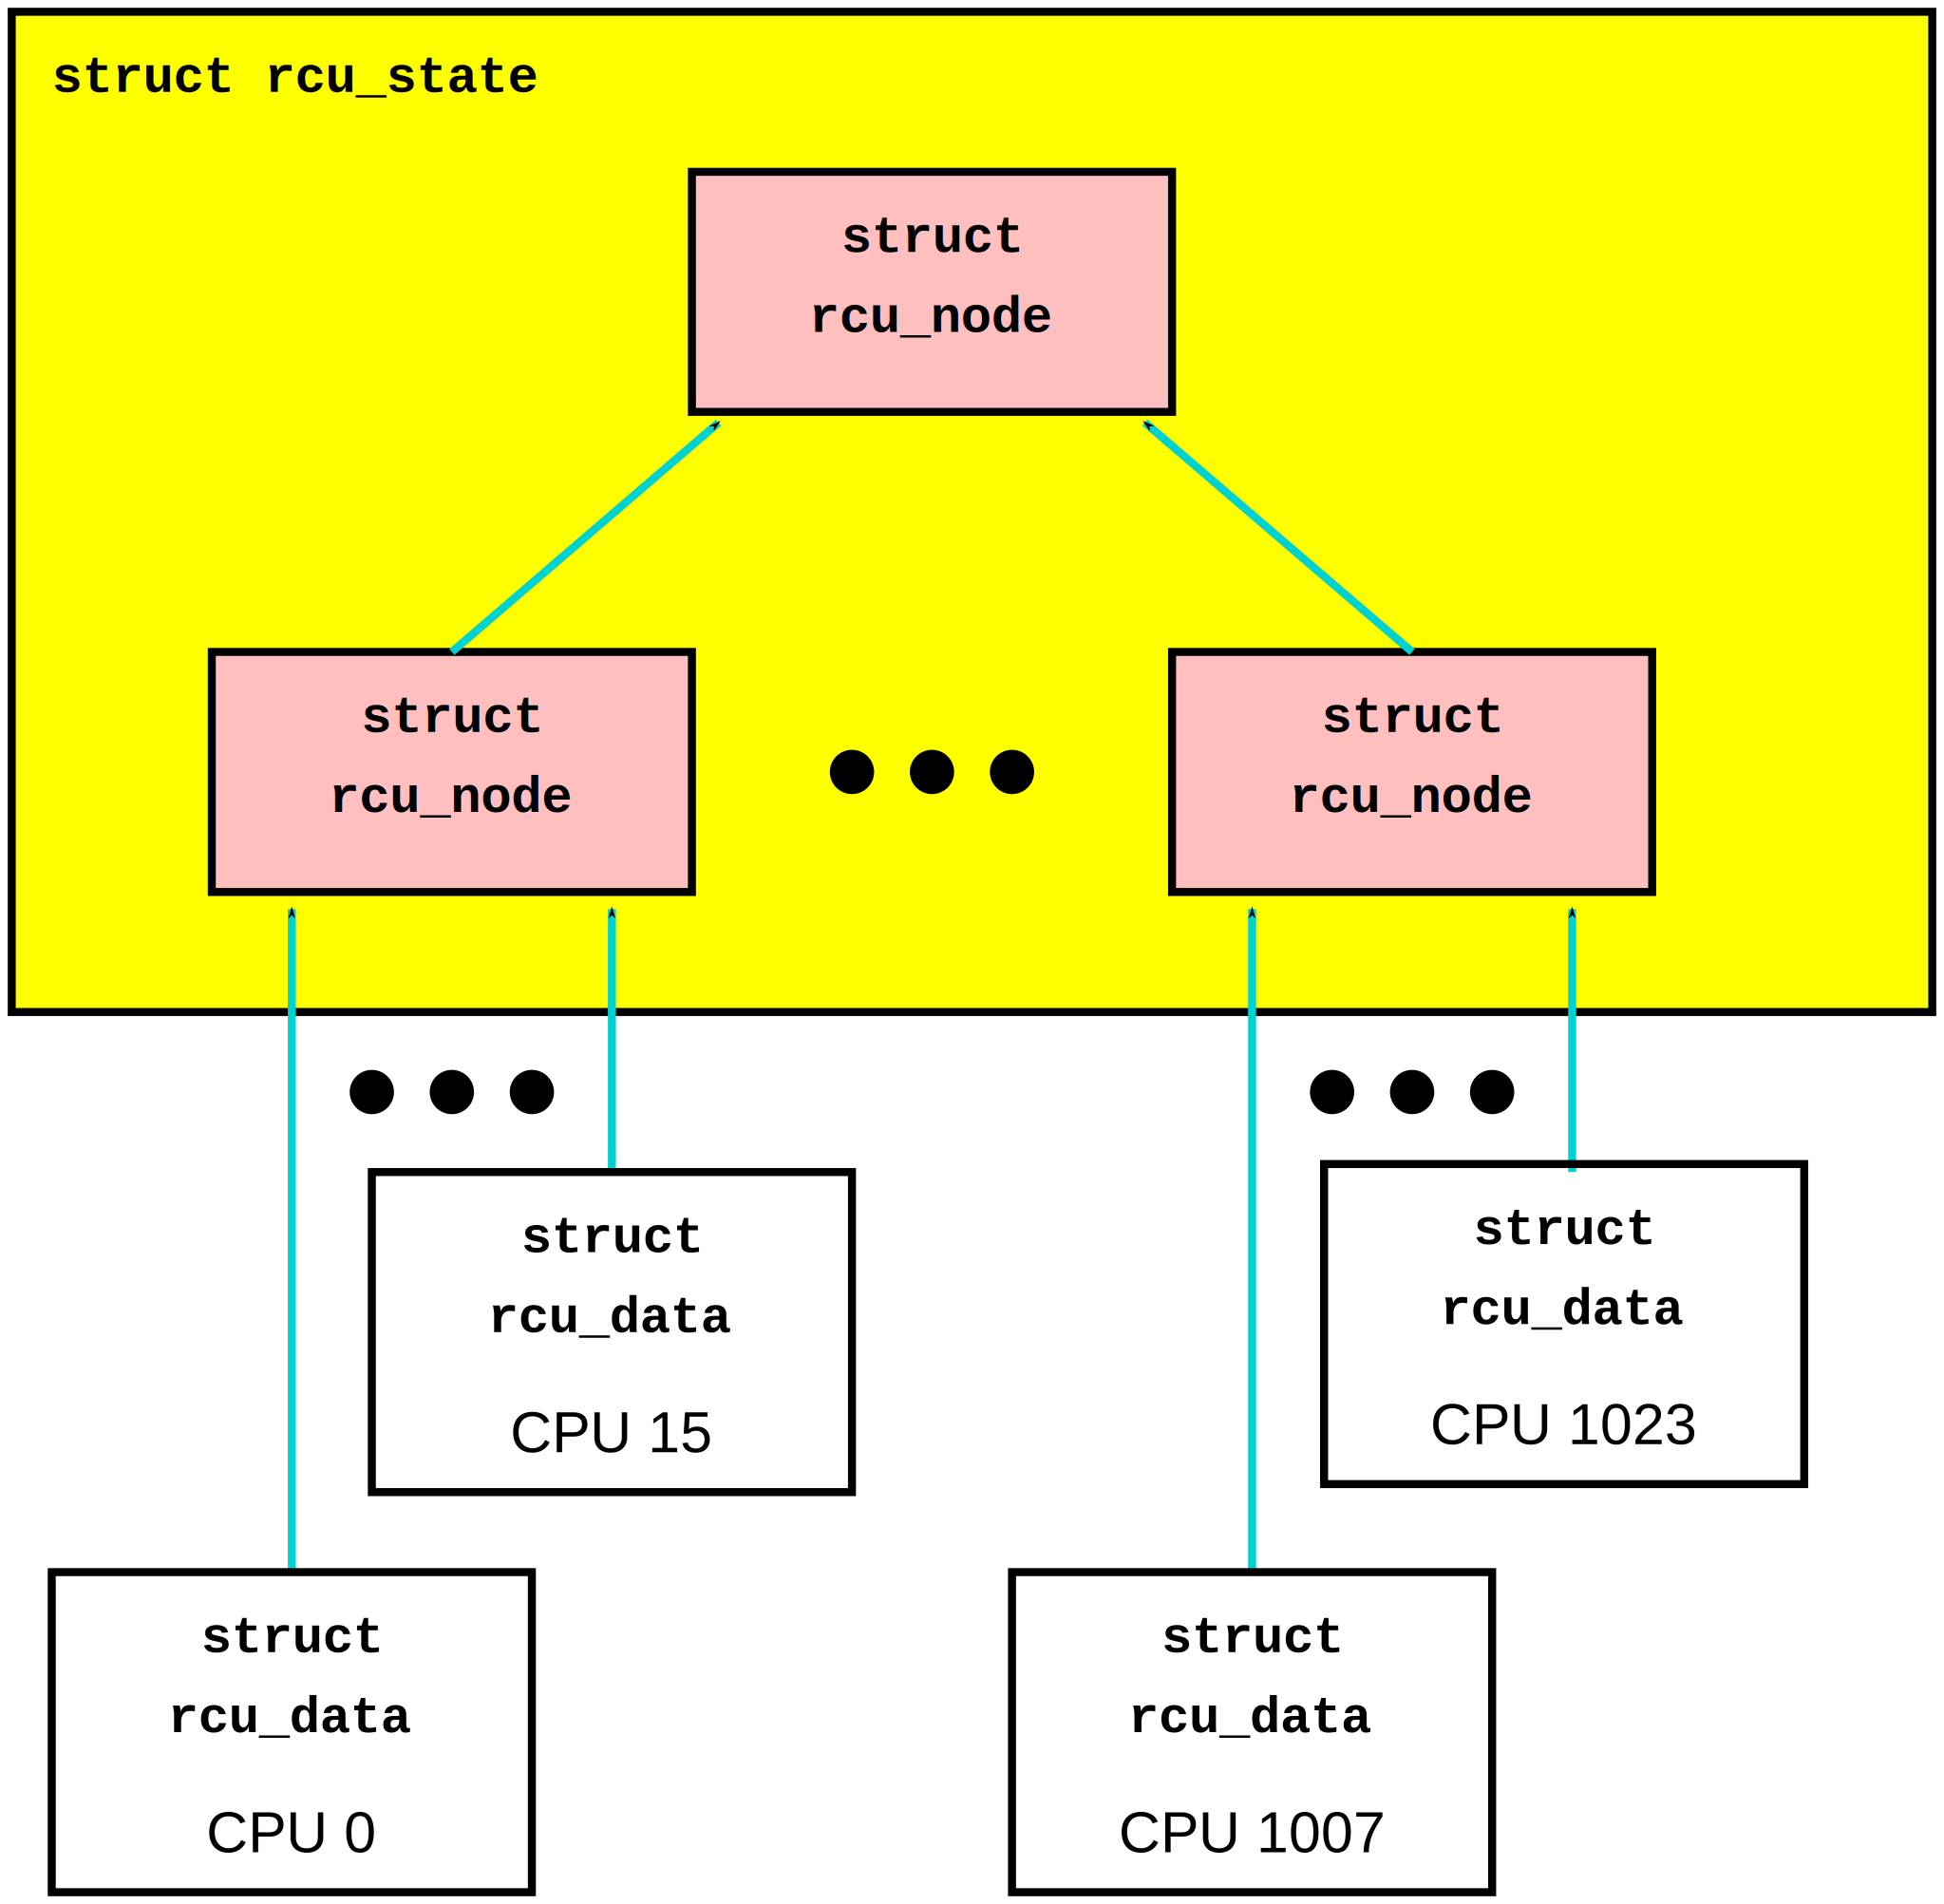
\includegraphics{rcu/design/BigTreeClassicRCU}}
\end{center}

This diagram shows an enclosing \co{rcu_state} structure containing a tree
of \co{rcu_node} structures.
Each leaf node of the \co{rcu_node} tree has up
to 16 \co{rcu_data} structures associated with it, so that there are
\co{NR_CPUS} number of \co{rcu_data} structures, one for each possible CPU\@.
This structure is adjusted at boot time, if needed, to handle the common
case where \co{nr_cpu_ids} is much less than \co{NR_CPUs}.
For example, a number of Linux distributions set \co{NR_CPUs=4096},
which results in a three-level \co{rcu_node} tree.
If the actual hardware has only 16 CPUs, RCU will adjust itself
at boot time, resulting in an \co{rcu_node} tree with only a single node.

The purpose of this combining tree is to allow per-CPU events
such as quiescent states, dyntick-idle transitions,
and CPU hotplug operations to be processed efficiently
and scalably.
Quiescent states are recorded by the per-CPU \co{rcu_data} structures,
and other events are recorded by the leaf-level \co{rcu_node}
structures.
All of these events are combined at each level of the tree until finally
grace periods are completed at the tree's root \co{rcu_node}
structure.
A grace period can be completed at the root once every CPU
(or, in the case of \co{CONFIG_PREEMPT_RCU}, task)
has passed through a quiescent state.
Once a grace period has completed, record of that fact is propagated
back down the tree.

As can be seen from the diagram, on a 64-bit system
a two-level tree with 64 leaves can accommodate 1,024 CPUs, with a fanout
of 64 at the root and a fanout of 16 at the leaves.

\QuickQuiz{
  Why isn't the fanout at the leaves also 64?
}\QuickQuizAnswer{
  Because there are more types of events that affect the leaf-level
  \co{rcu_node} structures than further up the tree.
  Therefore, if the
  leaf \co{rcu_node} structures have fanout of 64, the contention on
  these structures' \co{->structures} becomes excessive.
  Experimentation
  on a wide variety of systems has shown that a fanout of 16 works well
  for the leaves of the \co{rcu_node} tree.

  Of course, further experience with systems having hundreds or
  thousands of CPUs may demonstrate that the fanout for the non-leaf
  \co{rcu_node} structures must also be reduced.
  Such reduction can be
  easily carried out when and if it proves necessary.
  In the meantime,
  if you are using such a system and running into contention problems
  on the non-leaf \co{rcu_node} structures, you may use the
  \co{CONFIG_RCU_FANOUT} kernel configuration parameter to reduce the
  non-leaf fanout as needed.

  Kernels built for systems with strong NUMA characteristics might
  also need to adjust \co{CONFIG_RCU_FANOUT} so that the domains of
  the \co{rcu_node} structures align with hardware boundaries.
  However, there has thus far been no need for this.
}\QuickQuizEnd

If your system has more than 1,024 CPUs (or more than 512 CPUs on a
32-bit system), then RCU will automatically add more levels to the tree.
For example, if you are crazy enough to build a 64-bit system with
65,536 CPUs, RCU would configure the \co{rcu_node} tree as follows:

\begin{center}
\resizebox{\columnwidth}{!}{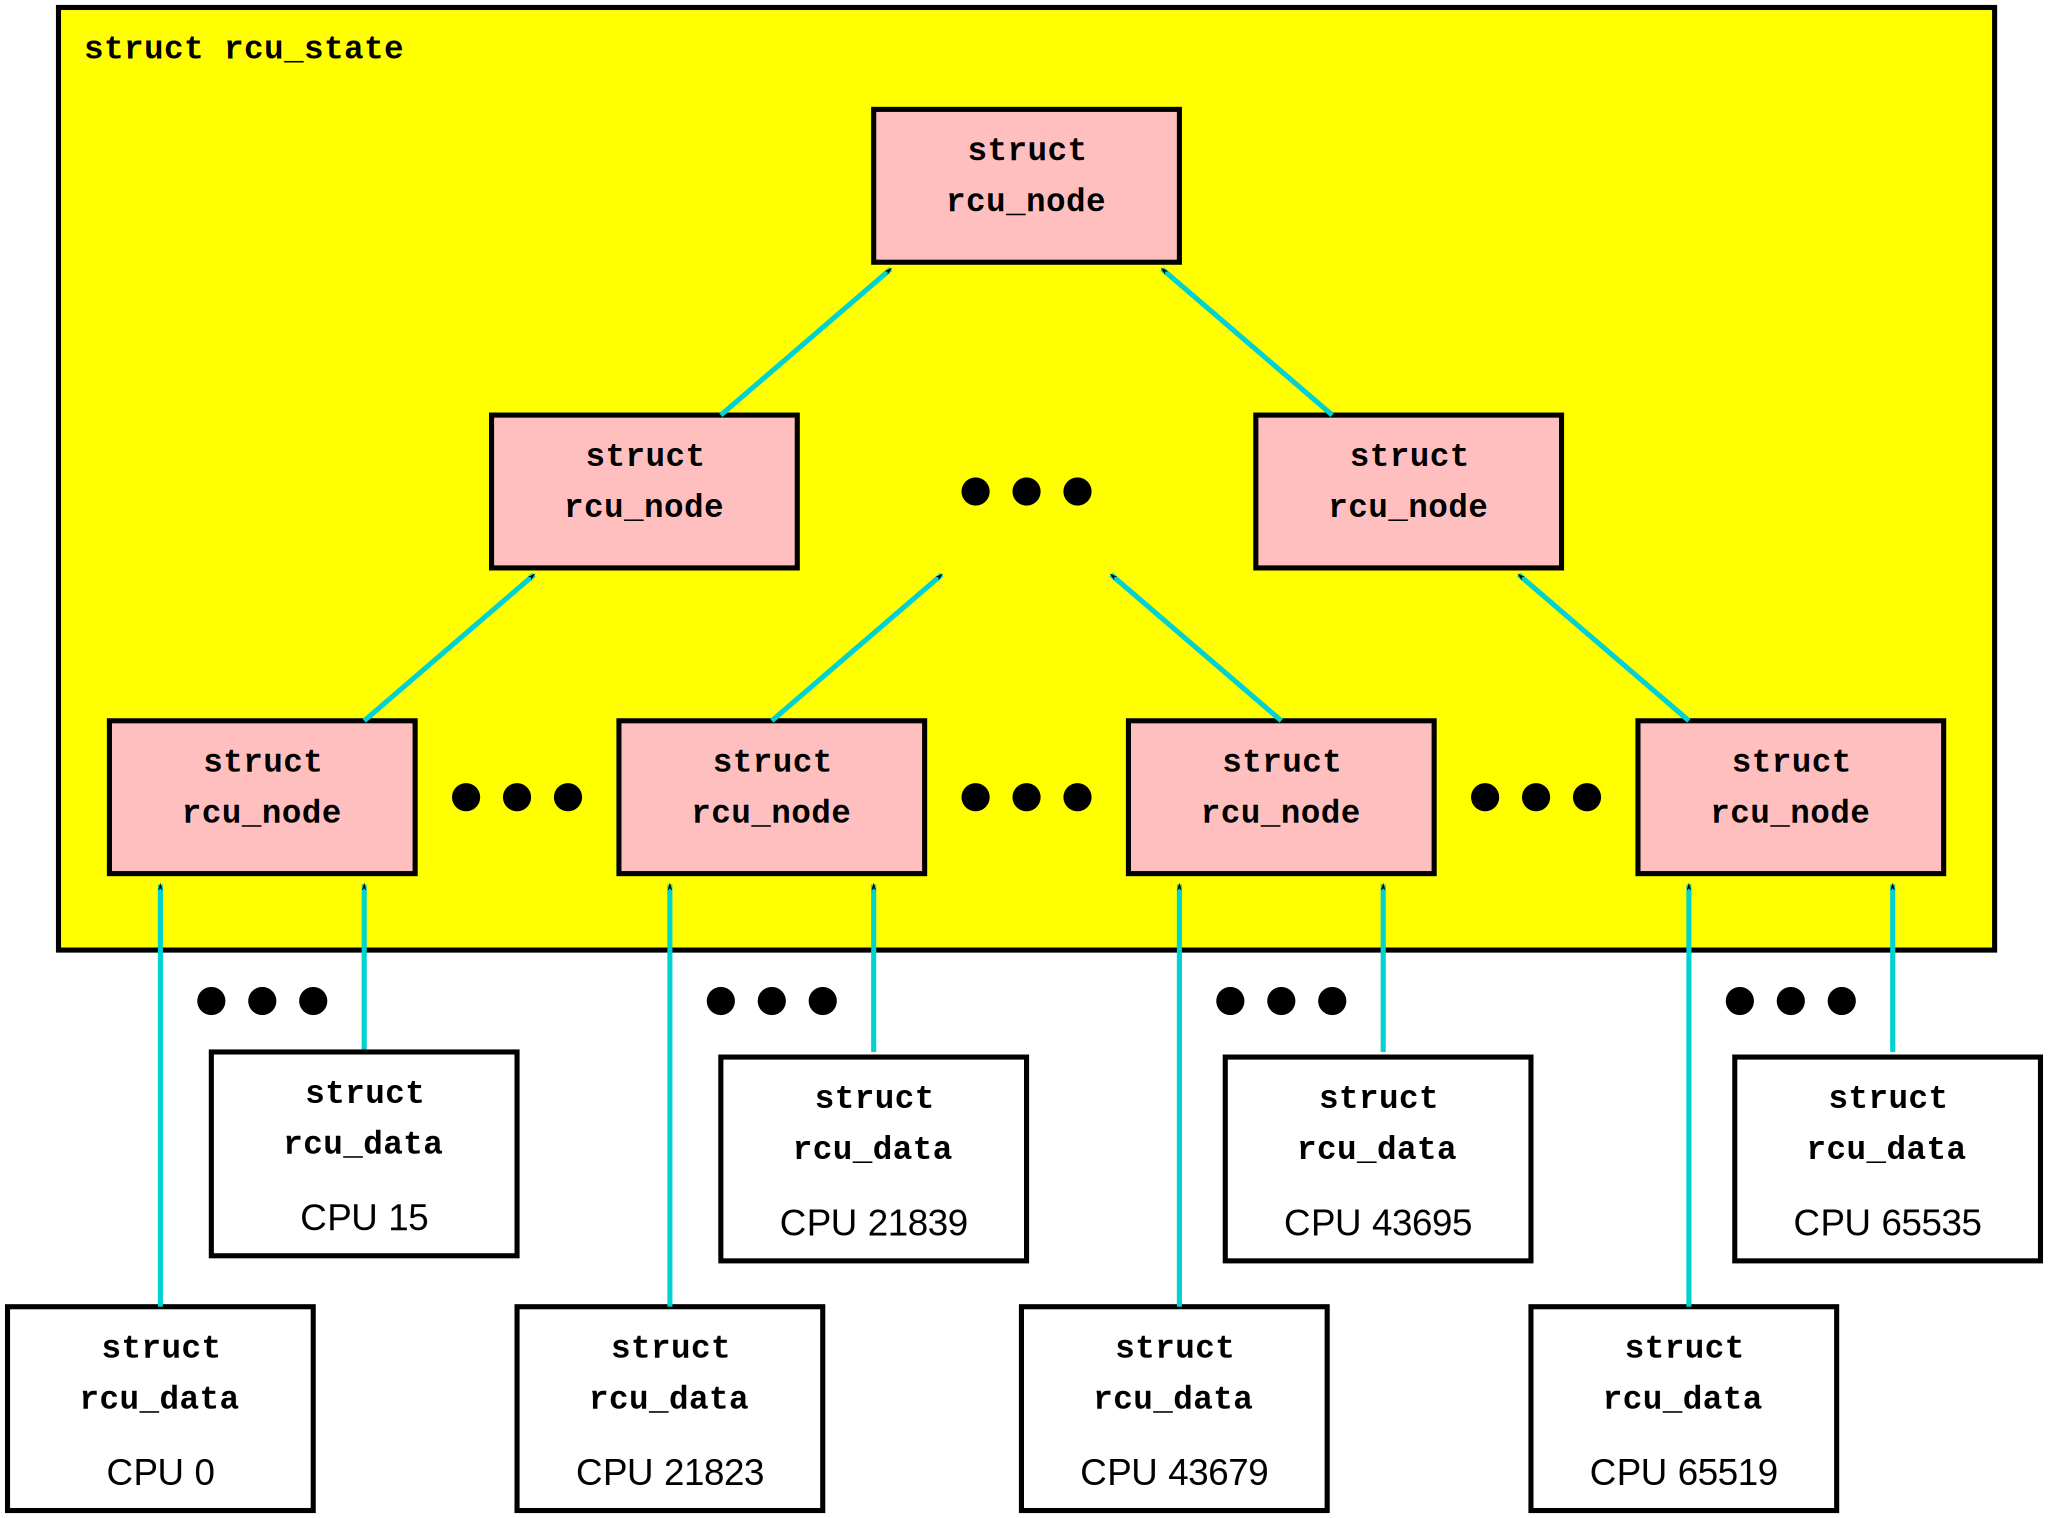
\includegraphics{rcu/design/HugeTreeClassicRCU}}
\end{center}

RCU currently permits up to a four-level tree, which on a 64-bit system
accommodates up to 4,194,304 CPUs, though only a mere 524,288 CPUs for
32-bit systems.
On the other hand, you can set both
\co{CONFIG_RCU_FANOUT} and \co{CONFIG_RCU_FANOUT_LEAF} to be as small as~2,
which would result in a 16-CPU test using a 4-level tree.
This can be
useful for testing large-system capabilities on small test machines.

This multi-level combining tree allows us to get most of the performance
and scalability benefits of partitioning, even though RCU grace-period
detection is inherently a global operation.
The trick here is that only
the last CPU to report a quiescent state into a given \co{rcu_node}
structure need advance to the \co{rcu_node} structure at the next level
up the tree.
This means that at the leaf-level \co{rcu_node} structure,
only one access out of sixteen will progress up the tree.
For the
internal \co{rcu_node} structures, the situation is even more extreme:
Only one access out of sixty-four will progress up the tree.
Because the
vast majority of the CPUs do not progress up the tree, the lock
contention remains roughly constant up the tree.
No matter how many CPUs
there are in the system, at most 64 quiescent-state reports per grace
period will progress all the way to the root \co{rcu_node} structure,
thus ensuring that the lock contention on that root \co{rcu_node}
structure remains acceptably low.

In effect, the combining tree acts like a big shock absorber, keeping
lock contention under control at all tree levels regardless of the level
of loading on the system.

RCU updaters wait for normal grace periods by registering RCU callbacks,
either directly via \co{call_rcu()} or indirectly via
\co{synchronize_rcu()} and friends.
RCU callbacks are represented by
\co{rcu_head} structures, which are queued on \co{rcu_data} structures
while they are waiting for a grace period to elapse, as shown in the
following figure:

\begin{center}
\resizebox{.8\columnwidth}{!}{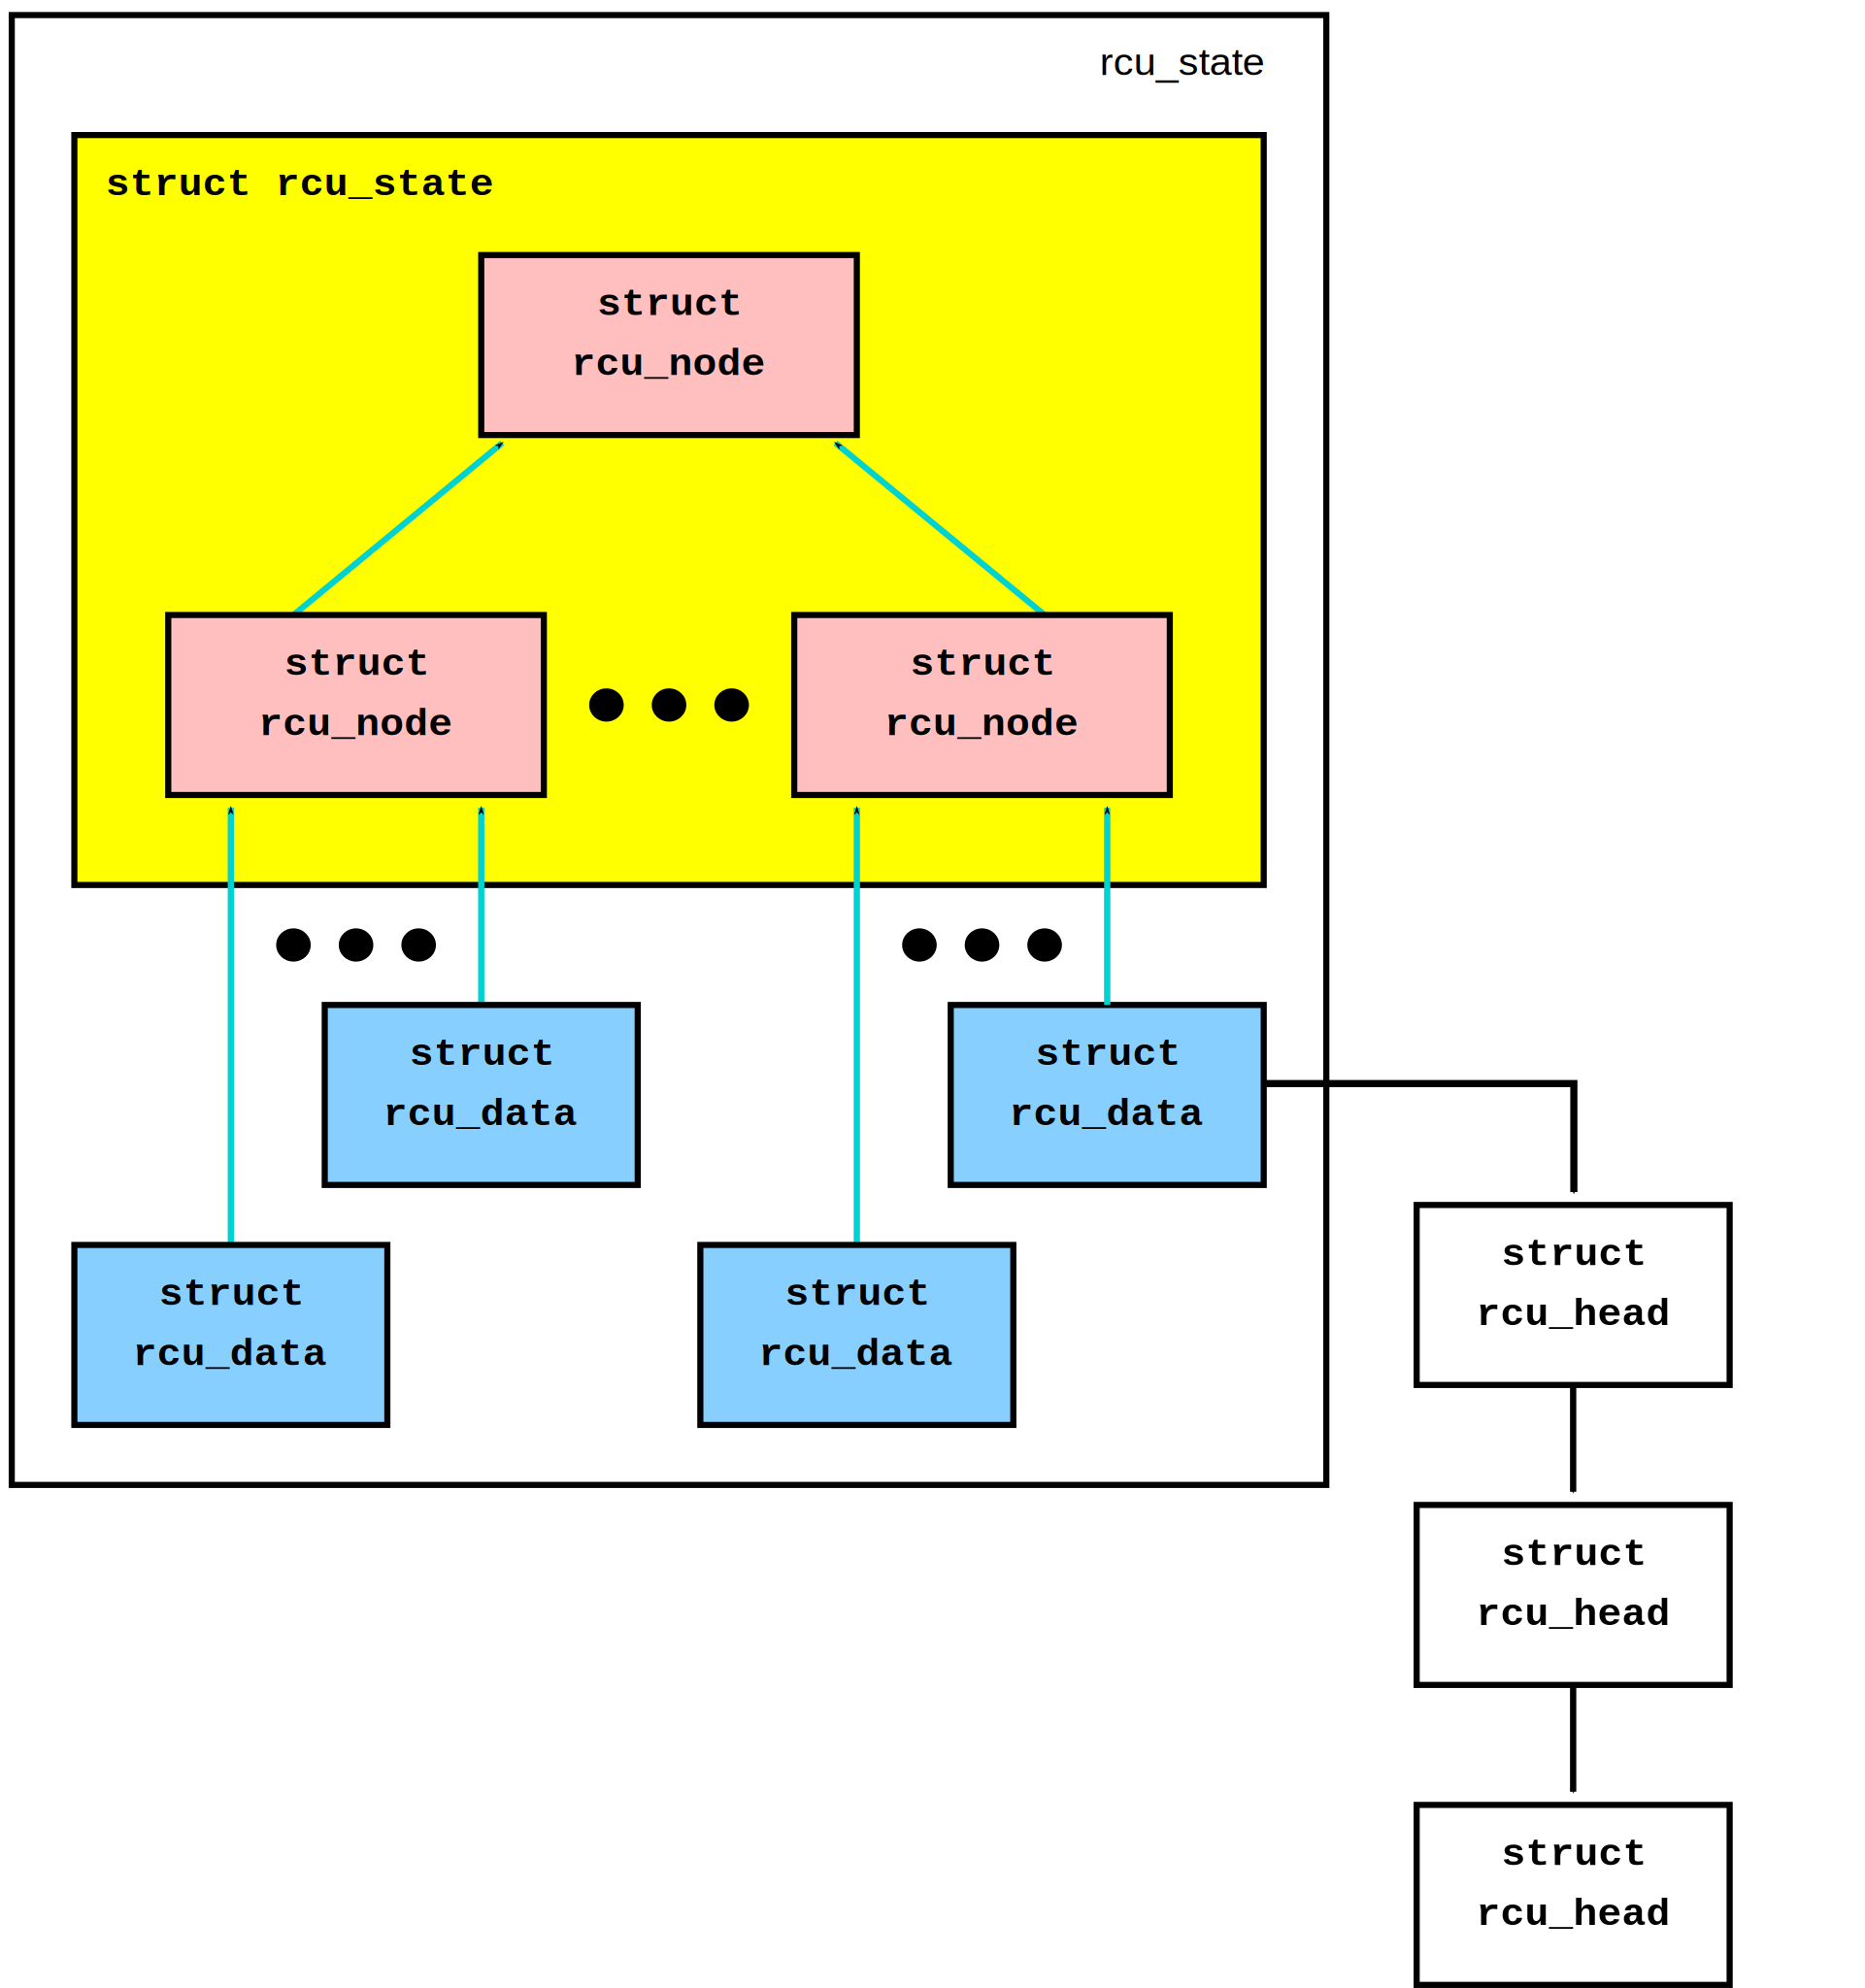
\includegraphics{rcu/design/BigTreePreemptRCUBHdyntickCB}}
\end{center}

This figure shows how \co{TREE_RCU}'s and \co{PREEMPT_RCU}'s major data
structures are related.
Lesser data structures will be introduced with
the algorithms that make use of them.

Note that each of the data structures in the above figure has its own
synchronization:

\begin{enumerate}
\item Each \co{rcu_state} structures has a lock and a mutex, and some fields
   are protected by the corresponding root \co{rcu_node} structure's lock.
\item Each \co{rcu_node} structure has a spinlock.
\item The fields in \co{rcu_data} are private to the corresponding CPU,
   although a few can be read and written by other CPUs.
\end{enumerate}

It is important to note that different data structures can have very
different ideas about the state of RCU at any given time.
For but one
example, awareness of the start or end of a given RCU grace period
propagates slowly through the data structures.
This slow propagation is
absolutely necessary for RCU to have good read-side performance.
If this
balkanized implementation seems foreign to you, one useful trick is to
consider each instance of these data structures to be a different
person, each having the usual slightly different view of reality.

The general role of each of these data structures is as follows:

\begin{description}
\item[\tco{rcu_state}:]
   This structure forms the interconnection between the
   \co{rcu_node} and \co{rcu_data} structures, tracks grace periods,
   serves as short-term repository for callbacks orphaned by CPU-hotplug
   events, maintains \co{rcu_barrier()} state, tracks expedited
   grace-period state, and maintains state used to force quiescent
   states when grace periods extend too long,
\item[\tco{rcu_node}:]
   This structure forms the combining tree that propagates
   quiescent-state information from the leaves to the root, and also
   propagates grace-period information from the root to the leaves.
   It
   provides local copies of the grace-period state in order to allow
   this information to be accessed in a synchronized manner without
   suffering the scalability limitations that would otherwise be imposed
   by global locking.
   In \co{CONFIG_PREEMPT_RCU} kernels, it manages the
   lists of tasks that have blocked while in their current RCU read-side
   critical section.
   In \co{CONFIG_PREEMPT_RCU} with
   \co{CONFIG_RCU_BOOST}, it manages the per-\co{rcu_node}
   priority-boosting kernel threads (kthreads) and state.
   Finally, it
   records CPU-hotplug state in order to determine which CPUs should be
   ignored during a given grace period.
\item[\tco{rcu_data}:]
   This per-CPU structure is the focus of quiescent-state
   detection and RCU callback queuing.
   It also tracks its relationship
   to the corresponding leaf \co{rcu_node} structure to allow
   more-efficient propagation of quiescent states up the \co{rcu_node}
   combining tree.
   Like the \co{rcu_node} structure, it provides a local
   copy of the grace-period information to allow for-free synchronized
   access to this information from the corresponding CPU\@.
   Finally, this
   structure records past dyntick-idle state for the corresponding CPU
   and also tracks statistics.
\item[\tco{rcu_head}:] This structure represents RCU callbacks, and is the
   only structure allocated and managed by RCU users.
   The \co{rcu_head}
   structure is normally embedded within the RCU-protected data
   structure.
\end{description}

If all you wanted from this article was a general notion of how RCU's
data structures are related, you are done.
Otherwise, each of the
following sections give more details on the \co{rcu_state}, \co{rcu_node}
and \co{rcu_data} data structures.

\subsubsection{The \texttt{rcu\_state} Structure}

The \co{rcu_state} structure is the base structure that represents the
state of RCU in the system.
This structure forms the interconnection
between the \co{rcu_node} and \co{rcu_data} structures, tracks grace
periods, contains the lock used to synchronize with CPU-hotplug events,
and maintains state used to force quiescent states when grace periods
extend too long.

A few of the \co{rcu_state} structure's fields are discussed, singly and
in groups, in the following sections. The more specialized fields are
covered in the discussion of their use.

\paragraph{Relationship to \texttt{rcu\_node} and \texttt{rcu\_data} Structures}

This portion of the \co{rcu_state} structure is declared as follows:

\begin{VerbatimN}
		struct rcu_node node[NUM_RCU_NODES];
		struct rcu_node *level[NUM_RCU_LVLS + 1];
		struct rcu_data __percpu *rda;
\end{VerbatimN}

\QuickQuiz{
  Wait a minute!
  You said that the \co{rcu_node} structures formed a
  tree, but they are declared as a flat array!
  What gives?
}\QuickQuizAnswer{
  The tree is laid out in the array.
  The first node In the array is the
  head, the next set of nodes in the array are children of the head
  node, and so on until the last set of nodes in the array are the
  leaves.
  See the diagrams following this Quick Quiz to see how this works.
}\QuickQuizEnd

The \co{rcu_node} tree is embedded into the \co{->node[]} array as shown
in the following figure:

\begin{center}
\resizebox{.8\columnwidth}{!}{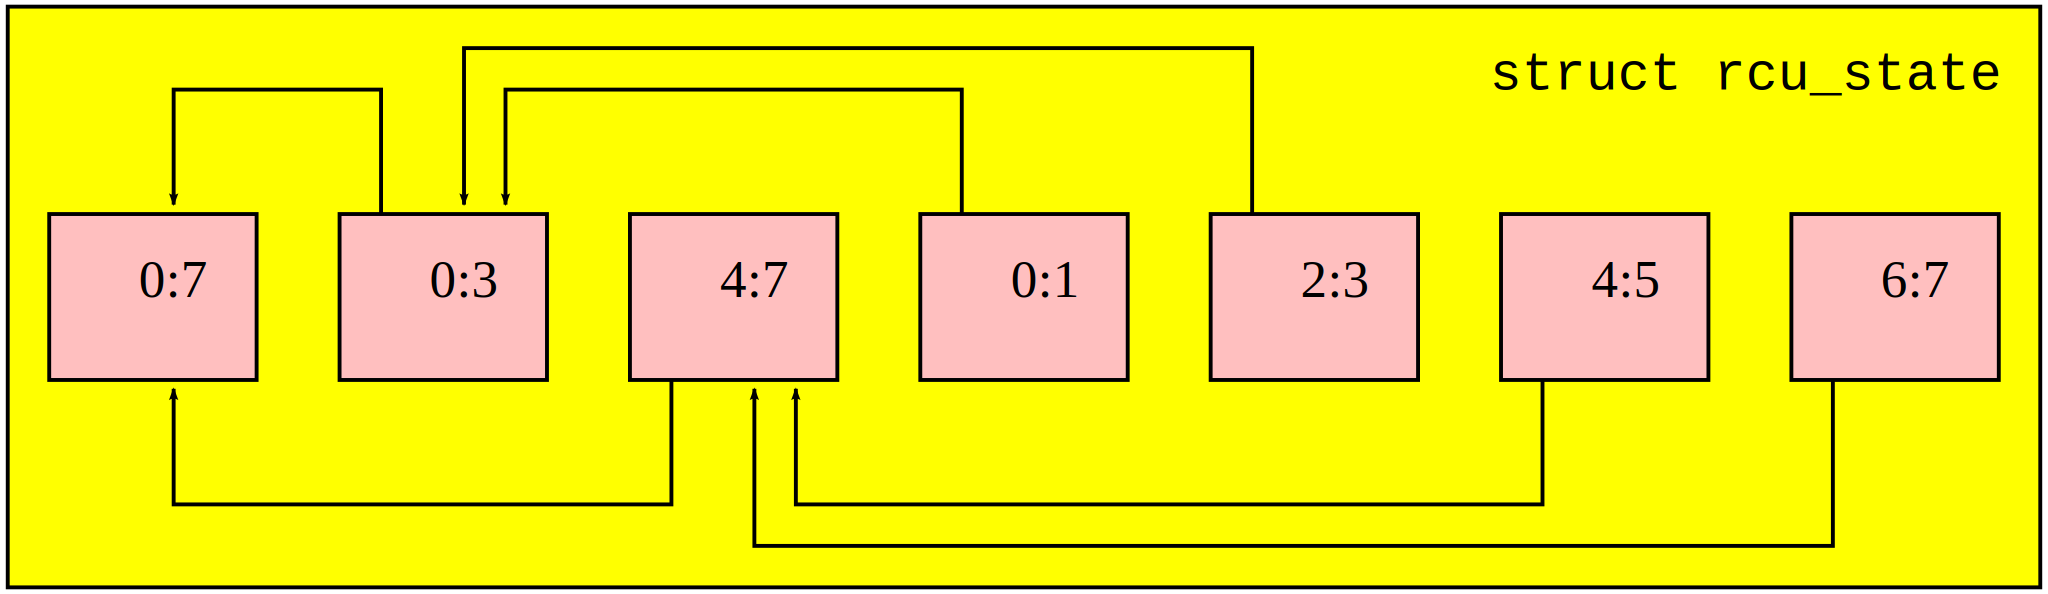
\includegraphics{rcu/design/TreeMapping}}
\end{center}

One interesting consequence of this mapping is that a breadth-first
traversal of the tree is implemented as a simple linear scan of the
array, which is in fact what the \co{rcu_for_each_node_breadth_first()}
macro does.
This macro is used at the beginning and ends of grace
periods.

Each entry of the \co{->level} array references the first \co{rcu_node}
structure on the corresponding level of the tree, for example, as shown
below:

\begin{center}
\resizebox{.8\columnwidth}{!}{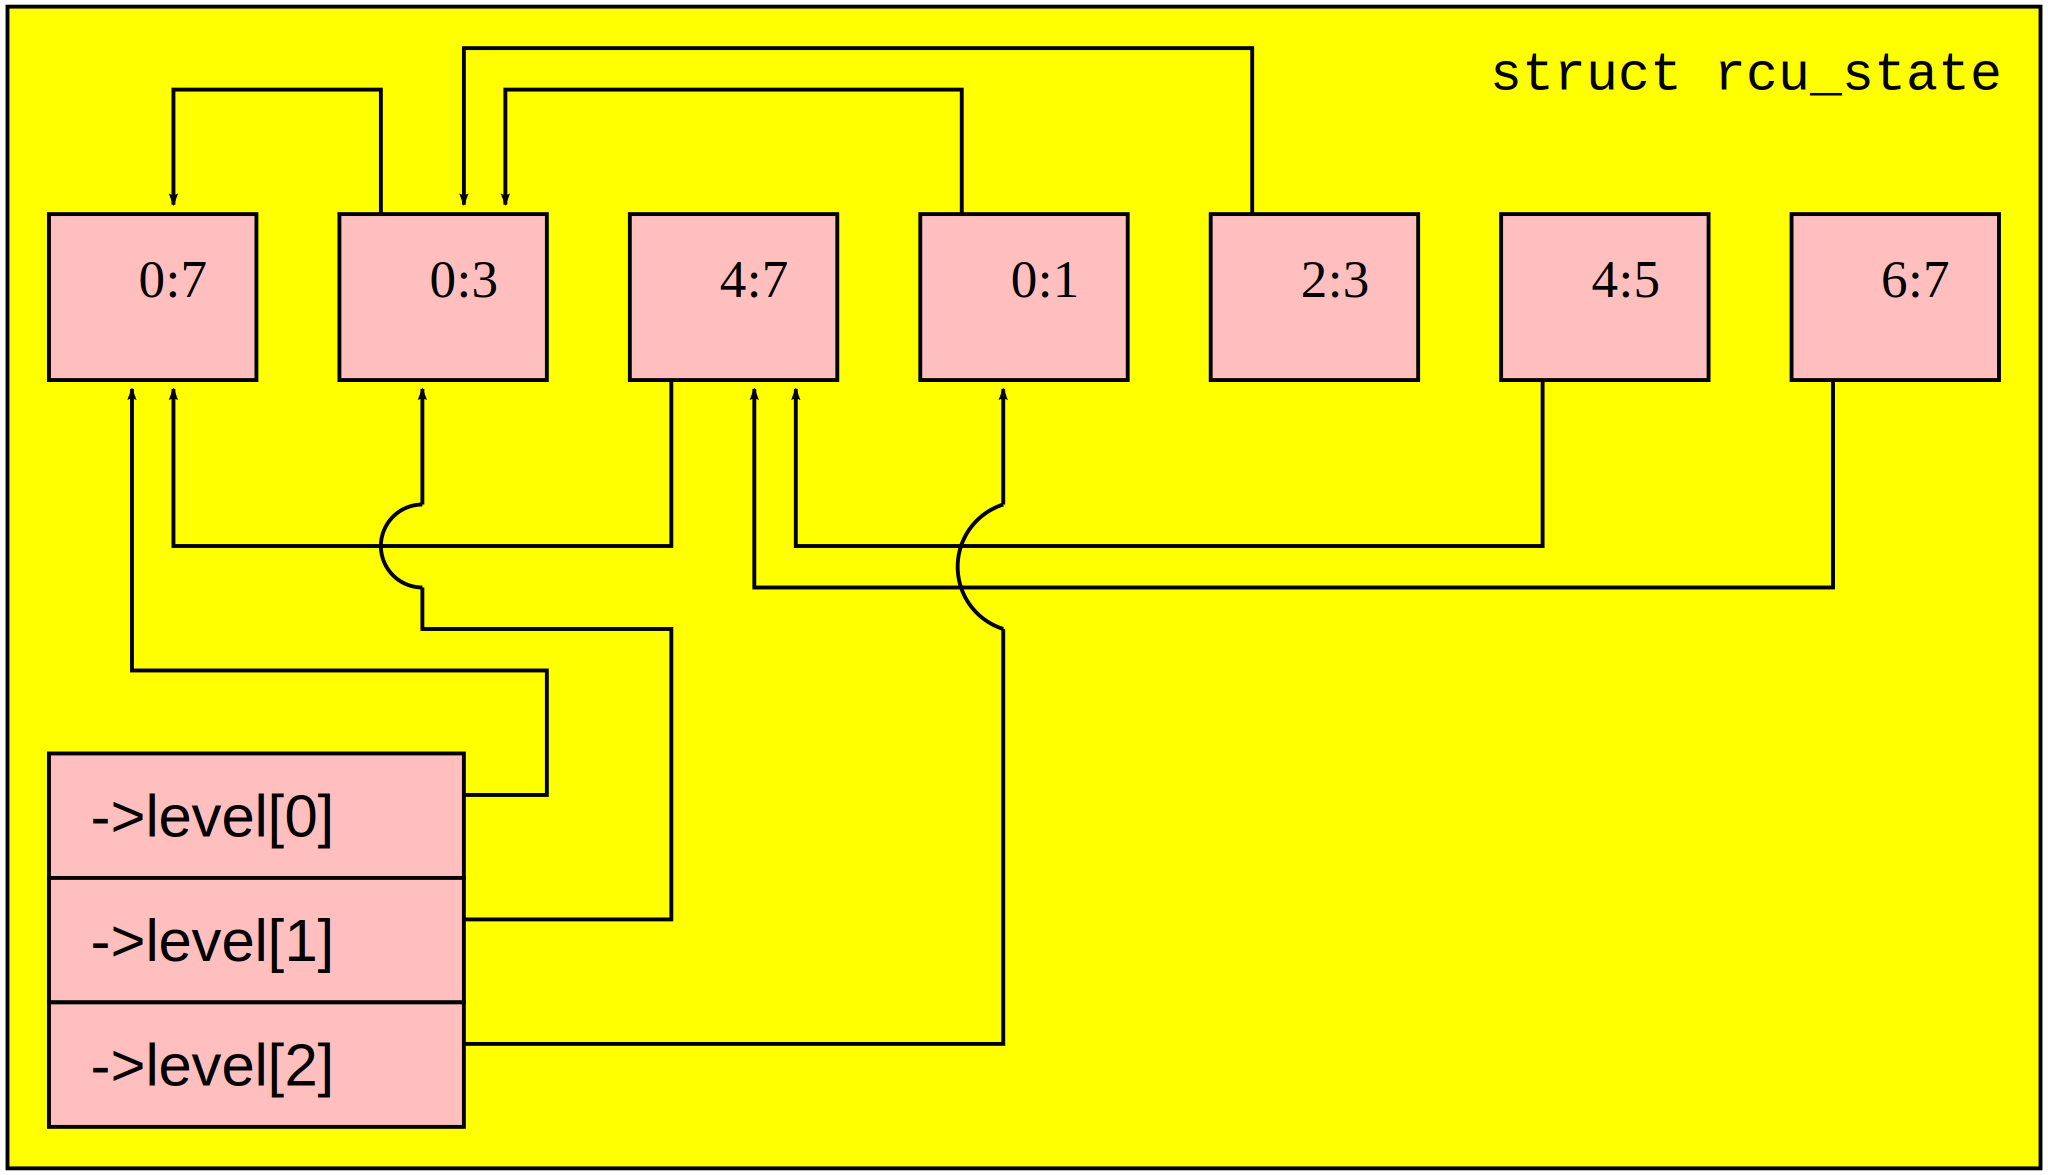
\includegraphics{rcu/design/TreeMappingLevel}}
\end{center}

The zero\textsuperscript{th} element of the array references the root
\co{rcu_node} structure, the first element references the first child of
the root \co{rcu_node}, and finally the second element references the
first leaf \co{rcu_node} structure.

For whatever it is worth, if you draw the tree to be tree-shaped rather
than array-shaped, it is easy to draw a planar representation:

\begin{center}
\resizebox{\columnwidth}{!}{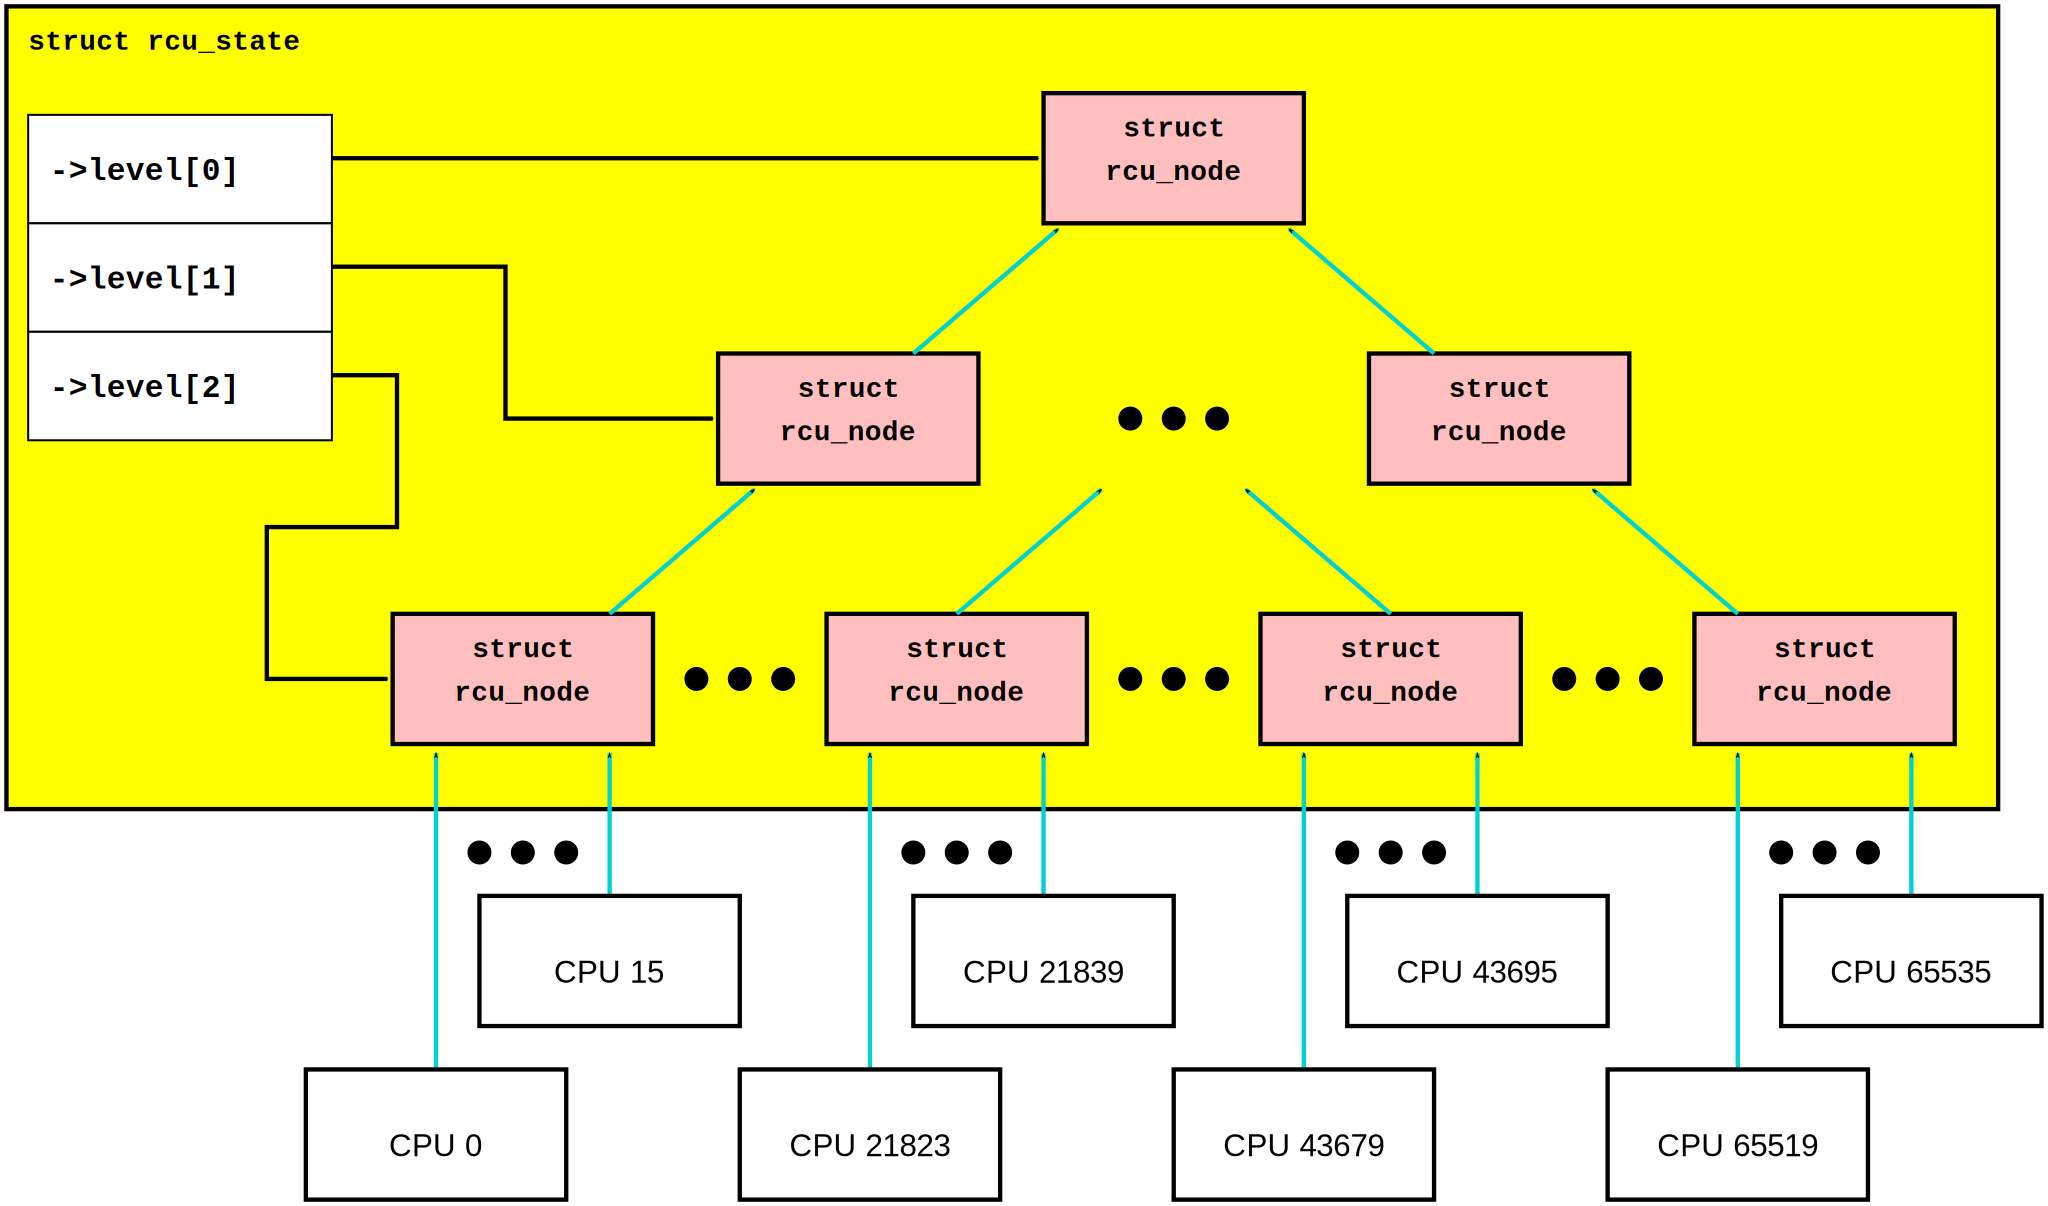
\includegraphics{rcu/design/TreeLevel}}
\end{center}

Finally, the \co{->rda} field references a per-CPU pointer to the
corresponding CPU's \co{rcu_data} structure.

All of these fields are constant once initialization is complete, and
therefore need no protection.

\paragraph{Grace-Period Tracking}

This portion of the \co{rcu_state} structure is declared as follows:

\begin{VerbatimN}
	unsigned long gp_seq;
\end{VerbatimN}

RCU grace periods are numbered, and the \co{->gp_seq} field contains the
current grace-period sequence number.
The bottom two bits are the state
of the current grace period, which can be zero for not yet started or
one for in progress. In other words, if the bottom two bits of
\co{->gp_seq} are zero, then RCU is idle. Any other value in the bottom
two bits indicates that something is broken.
This field is protected by
the root \co{rcu_node} structure's \co{->lock} field.

There are \co{->gp_seq} fields in the \co{rcu_node} and \co{rcu_data}
structures as well.
The fields in the \co{rcu_state} structure represent
the most current value, and those of the other structures are compared
in order to detect the beginnings and ends of grace periods in a
distributed fashion.
The values flow from \co{rcu_state} to \co{rcu_node}
(down the tree from the root to the leaves) to \co{rcu_data}.

\paragraph{Miscellaneous}

This portion of the \co{rcu_state} structure is declared as follows:

\begin{VerbatimN}
	unsigned long gp_max;
	char abbr;
	char *name;
\end{VerbatimN}

The \co{->gp_max} field tracks the duration of the longest grace period
in jiffies.
It is protected by the root \co{rcu_node}'s \co{->lock}.

The \co{->name} and \co{->abbr} fields distinguish between preemptible RCU
(\co{rcu_preempt} and \qco{p}) and non-preemptible RCU (\co{rcu_sched} and \qco{s}).
These fields are used for diagnostic and tracing purposes.

\subsubsection{The \texttt{rcu\_node} Structure}

The \co{rcu_node} structures form the combining tree that propagates
quiescent-state information from the leaves to the root and also that
propagates grace-period information from the root down to the leaves.
They provide local copies of the grace-period state in order to allow
this information to be accessed in a synchronized manner without
suffering the scalability limitations that would otherwise be imposed by
global locking.
In \co{CONFIG_PREEMPT_RCU} kernels, they manage the lists
of tasks that have blocked while in their current RCU read-side critical
section.
In \co{CONFIG_PREEMPT_RCU} with \co{CONFIG_RCU_BOOST}, they
manage the per-\co{rcu_node} priority-boosting kernel threads
(kthreads) and state.
Finally, they record CPU-hotplug state in order to
determine which CPUs should be ignored during a given grace period.

The \co{rcu_node} structure's fields are discussed, singly and in groups,
in the following sections.

\paragraph{Connection to Combining Tree}

This portion of the \co{rcu_node} structure is declared as follows:

\begin{VerbatimN}
	struct rcu_node *parent;
	u8 level;
	u8 grpnum;
	unsigned long grpmask;
	int grplo;
	int grphi;
\end{VerbatimN}

The \co{->parent} pointer references the \co{rcu_node} one level up in the
tree, and is \co{NULL} for the root \co{rcu_node}.
The RCU implementation
makes heavy use of this field to push quiescent states up the tree.
The
\co{->level} field gives the level in the tree, with the root being at
level zero, its children at level one, and so on.
The \co{->grpnum} field
gives this node's position within the children of its parent, so this
number can range between~0 and~31 on 32-bit systems and between~0 and~63
on 64-bit systems.
The \co{->level} and \co{->grpnum} fields are used only
during initialization and for tracing.
The \co{->grpmask} field is the
bitmask counterpart of \co{->grpnum}, and therefore always has exactly
one bit set.
This mask is used to clear the bit corresponding to this
\co{rcu_node} structure in its parent's bitmasks, which are described
later.
Finally, the \co{->grplo} and \co{->grphi} fields contain the
lowest and highest numbered CPU served by this \co{rcu_node} structure,
respectively.

All of these fields are constant, and thus do not require any
synchronization.

\paragraph{Synchronization}

This field of the \co{rcu_node} structure is declared as follows:

\begin{VerbatimN}
	raw_spinlock_t lock;
\end{VerbatimN}

This field is used to protect the remaining fields in this structure,
unless otherwise stated.
That said, all of the fields in this structure
can be accessed without locking for tracing purposes.
Yes, this can
result in confusing traces, but better some tracing confusion than to be
heisenbugged out of existence.

% .. _grace-period-tracking-1:

\paragraph{Grace-Period Tracking}

This portion of the \co{rcu_node} structure is declared as follows:

\begin{VerbatimN}
	unsigned long gp_seq;
	unsigned long gp_seq_needed;
\end{VerbatimN}

The \co{rcu_node} structures' \co{->gp_seq} fields are the counterparts of
the field of the same name in the \co{rcu_state} structure.
They each may
lag up to one step behind their \co{rcu_state} counterpart.
If the bottom
two bits of a given \co{rcu_node} structure's \co{->gp_seq} field is zero,
then this \co{rcu_node} structure believes that RCU is idle.

The \co{>gp_seq} field of each \co{rcu_node} structure is updated at the
beginning and the end of each grace period.

The \co{->gp_seq_needed} fields record the furthest-in-the-future grace
period request seen by the corresponding \co{rcu_node} structure.
The
request is considered fulfilled when the value of the \co{->gp_seq} field
equals or exceeds that of the \co{->gp_seq_needed} field.

\QuickQuiz{
  Suppose that this \co{rcu_node} structure doesn't see a request for a
  very long time.
  Won't wrapping of the \co{->gp_seq} field cause
  problems?
}\QuickQuizAnswer{
  No, because if the \co{->gp_seq_needed} field lags behind the
  \co{->gp_seq} field, the \co{->gp_seq_needed} field will be updated at
  the end of the grace period.
  Modulo-arithmetic comparisons therefore
  will always get the correct answer, even with wrapping.
}\QuickQuizEnd

\paragraph{Quiescent-State Tracking}

These fields manage the propagation of quiescent states up the combining
tree.

This portion of the \co{rcu_node} structure has fields as follows:

\begin{VerbatimN}
	unsigned long qsmask;
	unsigned long expmask;
	unsigned long qsmaskinit;
	unsigned long expmaskinit;
\end{VerbatimN}

The \co{->qsmask} field tracks which of this \co{rcu_node} structure's
children still need to report quiescent states for the current normal
grace period.
Such children will have a value of~1 in their
corresponding bit.
Note that the leaf \co{rcu_node} structures should be
thought of as having \co{rcu_data} structures as their children.
Similarly, the \co{->expmask} field tracks which of this \co{rcu_node}
structure's children still need to report quiescent states for the
current expedited grace period.
An expedited grace period has the same
conceptual properties as a normal grace period, but the expedited
implementation accepts extreme CPU overhead to obtain much lower
grace-period latency, for example, consuming a few tens of microseconds
worth of CPU time to reduce grace-period duration from milliseconds to
tens of microseconds.
The \co{->qsmaskinit} field tracks which of this
\co{rcu_node} structure's children cover for at least one online CPU\@.
This mask is used to initialize \co{->qsmask}, and \co{->expmaskinit} is
used to initialize \co{->expmask} and the beginning of the normal and
expedited grace periods, respectively.

\QuickQuiz{
  Why are these bitmasks protected by locking?
  Come on, haven't you
  heard of atomic instructions???
}\QuickQuizAnswer{
  Lockless grace-period computation!
  Such a tantalizing possibility!
  But consider the following sequence of events:

  \begin{enumerate}
  \item CPU~0 has been in dyntick-idle mode for quite some time.
     When it
     wakes up, it notices that the current RCU grace period needs it to
     report in, so it sets a flag where the scheduling clock interrupt
     will find it.
  \item Meanwhile, CPU~1 is running \co{force_quiescent_state()}, and
     notices that CPU~0 has been in dyntick idle mode, which qualifies
     as an extended quiescent state.
  \item CPU~0's scheduling clock interrupt fires in the middle of an RCU
     read-side critical section, and notices that the RCU core needs
     something, so commences RCU softirq processing.
  \item CPU~0's softirq handler executes and is just about ready to report
     its quiescent state up the \co{rcu_node} tree.
  \item But CPU~1 beats it to the punch, completing the current grace
     period and starting a new one.
  \item CPU~0 now reports its quiescent state for the wrong grace period.
     That grace period might now end before the RCU read-side critical
     section.
     If that happens, disaster will ensue.
  \end{enumerate}

  So the locking is absolutely required in order to coordinate clearing
  of the bits with updating of the grace-period sequence number in
  \co{->gp_seq}.
}\QuickQuizEnd

\paragraph{Blocked-Task Management}

\co{PREEMPT_RCU} allows tasks to be preempted in the midst of their RCU
read-side critical sections, and these tasks must be tracked explicitly.
The details of exactly why and how they are tracked will be covered in a
separate article on RCU read-side processing.
For now, it is enough to
know that the \co{rcu_node} structure tracks them.

\begin{VerbatimN}
	struct list_head blkd_tasks;
	struct list_head *gp_tasks;
	struct list_head *exp_tasks;
	bool wait_blkd_tasks;
\end{VerbatimN}

The \co{->blkd_tasks} field is a list header for the list of blocked and
preempted tasks.
As tasks undergo context switches within RCU read-side
critical sections, their \co{task_struct} structures are enqueued (via
the \co{task_struct}'s \co{->rcu_node_entry} field) onto the head of the
\co{->blkd_tasks} list for the leaf \co{rcu_node} structure corresponding
to the CPU on which the outgoing context switch executed.
As these tasks
later exit their RCU read-side critical sections, they remove themselves
from the list.
This list is therefore in reverse time order, so that if
one of the tasks is blocking the current grace period, all subsequent
tasks must also be blocking that same grace period.
Therefore, a single
pointer into this list suffices to track all tasks blocking a given
grace period.
That pointer is stored in \co{->gp_tasks} for normal grace
periods and in \co{->exp_tasks} for expedited grace periods.
These last
two fields are \co{NULL} if either there is no grace period in flight or
if there are no blocked tasks preventing that grace period from
completing.
If either of these two pointers is referencing a task that
removes itself from the \co{->blkd_tasks} list, then that task must
advance the pointer to the next task on the list, or set the pointer to
\co{NULL} if there are no subsequent tasks on the list.

For example, suppose that tasks~T1, T2, and~T3 are all hard-affinitied
to the largest-numbered CPU in the system.
Then if task~T1 blocked in an
RCU read-side critical section, then an expedited grace period started,
then task~T2 blocked in an RCU read-side critical section, then a normal
grace period started, and finally task~3 blocked in an RCU read-side
critical section, then the state of the last leaf \co{rcu_node}
structure's blocked-task list would be as shown below:

\begin{center}
\resizebox{\columnwidth}{!}{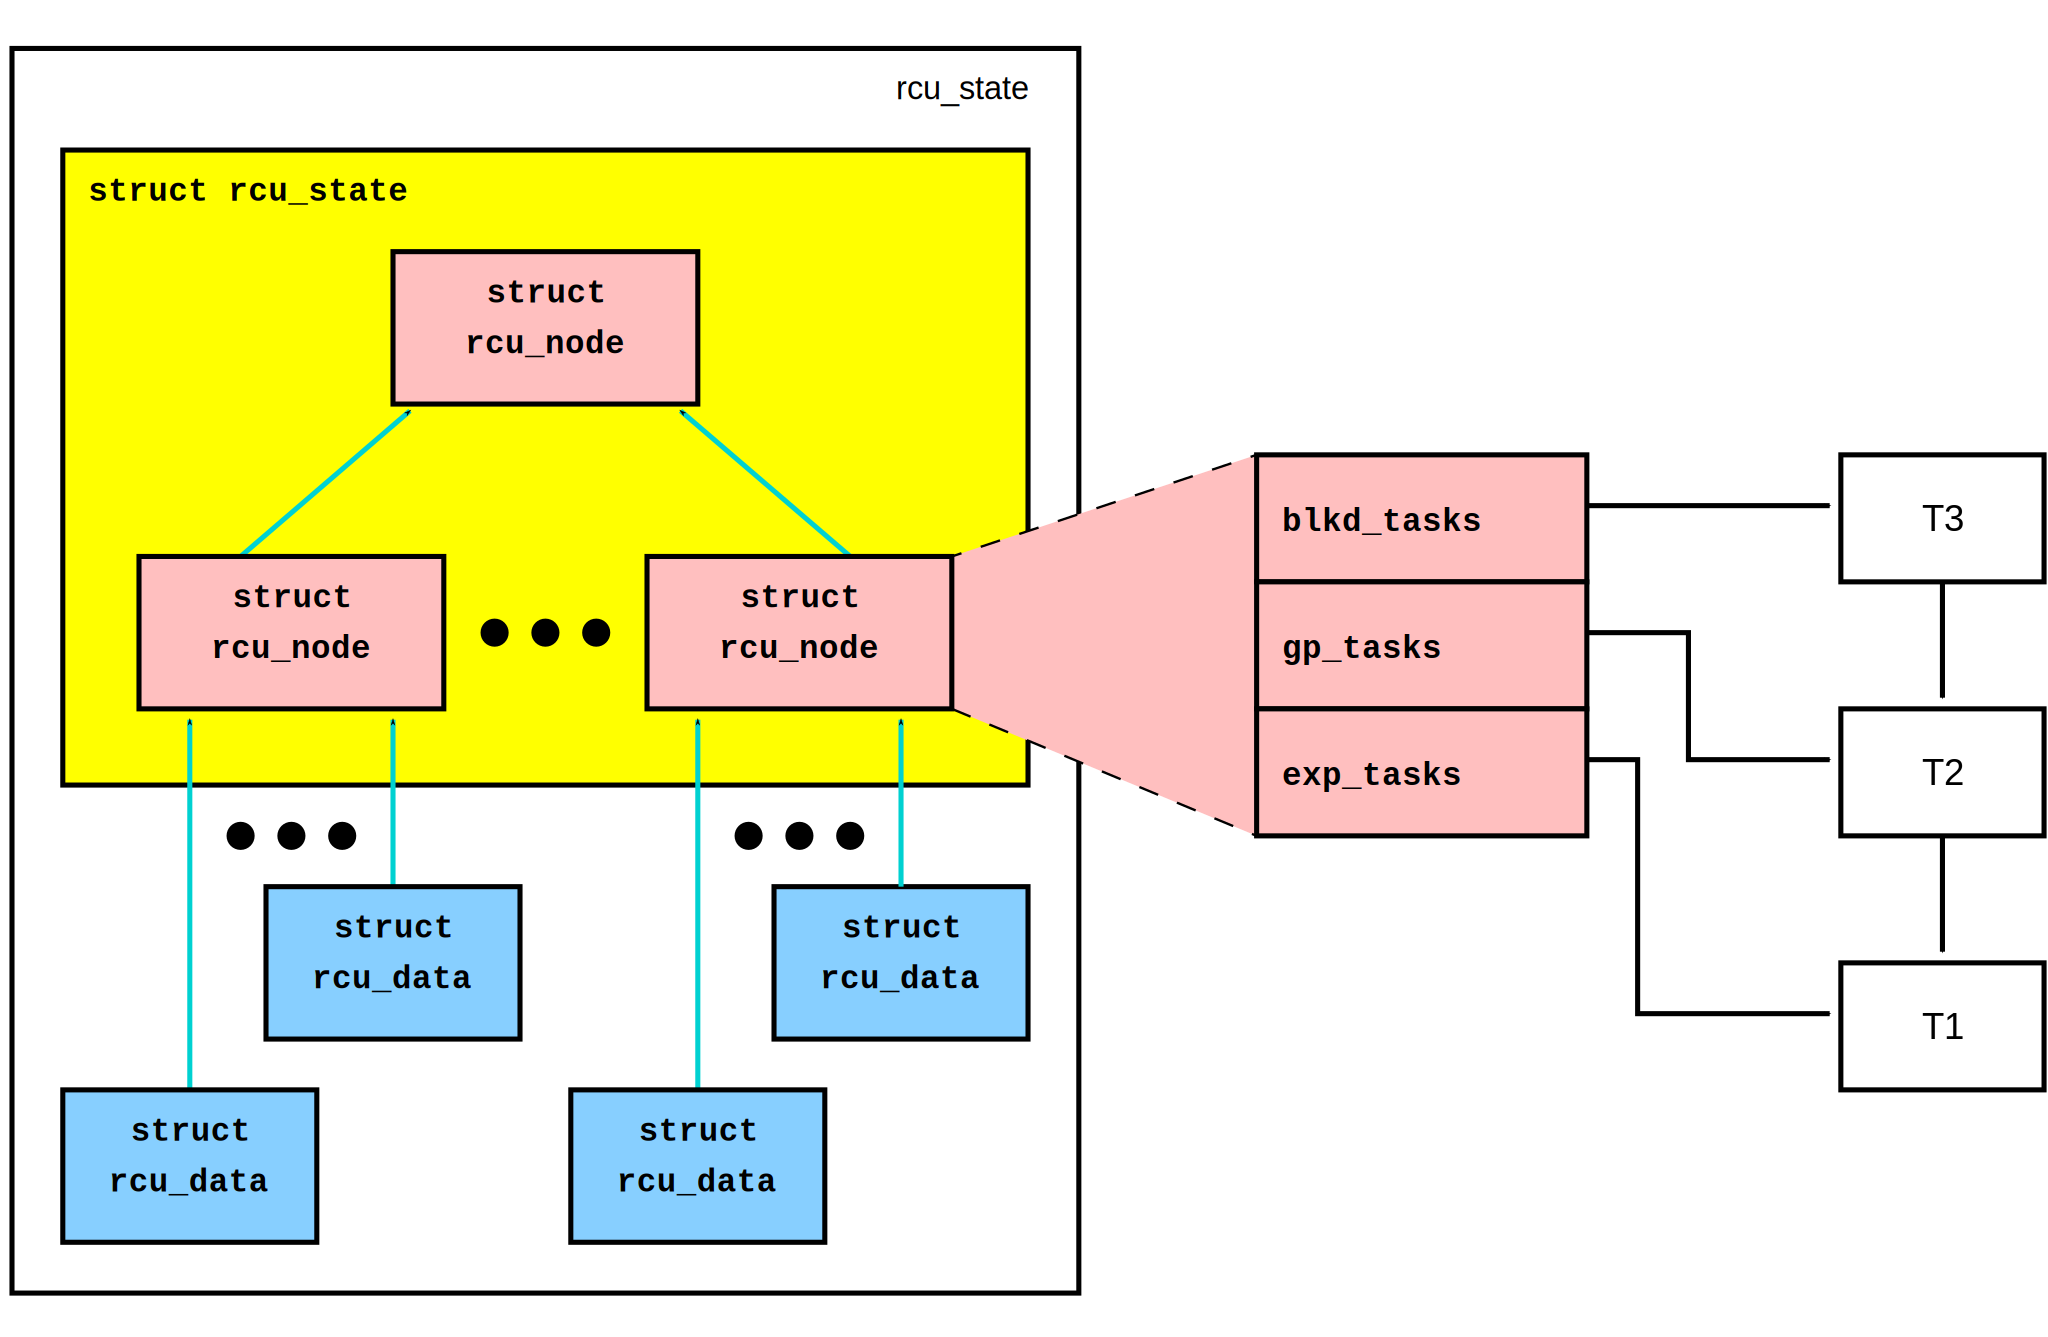
\includegraphics{rcu/design/blkd_task}}
\end{center}

Task~T1 is blocking both grace periods, task~T2 is blocking only the
normal grace period, and task~T3 is blocking neither grace period.
Note
that these tasks will not remove themselves from this list immediately
upon resuming execution.
They will instead remain on the list until they
execute the outermost \co{rcu_read_unlock()} that ends their RCU
read-side critical section.

The \co{->wait_blkd_tasks} field indicates whether or not the current
grace period is waiting on a blocked task.

\paragraph{Sizing the \texttt{rcu\_node} Array}

The \co{rcu_node} array is sized via a series of C-preprocessor
expressions as follows:

\begin{fcvlabel}[ln:rcu:design:data1]
\begin{VerbatimN}[breaklines=true,xleftmargin=1pt,xrightmargin=0pt,commandchars=\%\@\$]
	#ifdef CONFIG_RCU_FANOUT
	#define RCU_FANOUT CONFIG_RCU_FANOUT
	#else
	# ifdef CONFIG_64BIT
	# define RCU_FANOUT 64
	# else
	# define RCU_FANOUT 32
	# endif
	#endif

	#ifdef CONFIG_RCU_FANOUT_LEAF     %lnlbl@confleaf:if$
	#define RCU_FANOUT_LEAF CONFIG_RCU_FANOUT_LEAF
	#else
	# ifdef CONFIG_64BIT
	# define RCU_FANOUT_LEAF 64
	# else
	# define RCU_FANOUT_LEAF 32
	# endif
	#endif                            %lnlbl@confleaf:endif$

	#define RCU_FANOUT_1        (RCU_FANOUT_LEAF) %lnlbl@fanout1$
	#define RCU_FANOUT_2        (RCU_FANOUT_1 * RCU_FANOUT)
	#define RCU_FANOUT_3        (RCU_FANOUT_2 * RCU_FANOUT)
	#define RCU_FANOUT_4        (RCU_FANOUT_3 * RCU_FANOUT) %lnlbl@fanout4$

	#if NR_CPUS <= RCU_FANOUT_1       %lnlbl@cpus:if$
	#  define RCU_NUM_LVLS        1         %lnlbl@lvls1$
	#  define NUM_RCU_LVL_0        1        %lnlbl@lvl01$
	#  define NUM_RCU_NODES        NUM_RCU_LVL_0
	#  define NUM_RCU_LVL_INIT    { NUM_RCU_LVL_0 }
	#  define RCU_NODE_NAME_INIT  { "rcu_node_0" }  %lnlbl@nodenameinit1$
	#  define RCU_FQS_NAME_INIT   { "rcu_node_fqs_0" }
	#  define RCU_EXP_NAME_INIT   { "rcu_node_exp_0" }  %lnlbl@expnameinit1$
	#elif NR_CPUS <= RCU_FANOUT_2
	#  define RCU_NUM_LVLS        2         %lnlbl@lvls2$
	#  define NUM_RCU_LVL_0        1        %lnlbl@lvl02$
	#  define NUM_RCU_LVL_1        DIV_ROUND_UP(NR_CPUS, RCU_FANOUT_1) %lnlbl@lvl12$
	#  define NUM_RCU_NODES        (NUM_RCU_LVL_0 + NUM_RCU_LVL_1)
	#  define NUM_RCU_LVL_INIT    { NUM_RCU_LVL_0, NUM_RCU_LVL_1 }
	#  define RCU_NODE_NAME_INIT  { "rcu_node_0", "rcu_node_1" } %lnlbl@nodenameinit2$
	#  define RCU_FQS_NAME_INIT   { "rcu_node_fqs_0", "rcu_node_fqs_1" }
	#  define RCU_EXP_NAME_INIT   { "rcu_node_exp_0", "rcu_node_exp_1" } %lnlbl@expnameinit2$
	#elif NR_CPUS <= RCU_FANOUT_3
	#  define RCU_NUM_LVLS        3         %lnlbl@lvls3$
	#  define NUM_RCU_LVL_0        1        %lnlbl@lvl03$
	#  define NUM_RCU_LVL_1        DIV_ROUND_UP(NR_CPUS, RCU_FANOUT_2) %lnlbl@lvl13$
	#  define NUM_RCU_LVL_2        DIV_ROUND_UP(NR_CPUS, RCU_FANOUT_1) %lnlbl@lvl23$
	#  define NUM_RCU_NODES        (NUM_RCU_LVL_0 + NUM_RCU_LVL_1 + NUM_RCU_LVL_2)
	#  define NUM_RCU_LVL_INIT    { NUM_RCU_LVL_0, NUM_RCU_LVL_1, NUM_RCU_LVL_2 }
	#  define RCU_NODE_NAME_INIT  { "rcu_node_0", "rcu_node_1", "rcu_node_2" } %lnlbl@nodenameinit3$
	#  define RCU_FQS_NAME_INIT   { "rcu_node_fqs_0", "rcu_node_fqs_1", "rcu_node_fqs_2" }
	#  define RCU_EXP_NAME_INIT   { "rcu_node_exp_0", "rcu_node_exp_1", "rcu_node_exp_2" } %lnlbl@expnameinit3$
	#elif NR_CPUS <= RCU_FANOUT_4
	#  define RCU_NUM_LVLS        4         %lnlbl@lvls4$
	#  define NUM_RCU_LVL_0        1        %lnlbl@lvl04$
	#  define NUM_RCU_LVL_1        DIV_ROUND_UP(NR_CPUS, RCU_FANOUT_3) %lnlbl@lvl14$
	#  define NUM_RCU_LVL_2        DIV_ROUND_UP(NR_CPUS, RCU_FANOUT_2)
	#  define NUM_RCU_LVL_3        DIV_ROUND_UP(NR_CPUS, RCU_FANOUT_1) %lnlbl@lvl34$
	#  define NUM_RCU_NODES        (NUM_RCU_LVL_0 + NUM_RCU_LVL_1 + NUM_RCU_LVL_2 + NUM_RCU_LVL_3)
	#  define NUM_RCU_LVL_INIT    { NUM_RCU_LVL_0, NUM_RCU_LVL_1, NUM_RCU_LVL_2, NUM_RCU_LVL_3 }
	#  define RCU_NODE_NAME_INIT  { "rcu_node_0", "rcu_node_1", "rcu_node_2", "rcu_node_3" } %lnlbl@nodenameinit4$
	#  define RCU_FQS_NAME_INIT   { "rcu_node_fqs_0", "rcu_node_fqs_1", "rcu_node_fqs_2", "rcu_node_fqs_3" }
	#  define RCU_EXP_NAME_INIT   { "rcu_node_exp_0", "rcu_node_exp_1", "rcu_node_exp_2", "rcu_node_exp_3" }  %lnlbl@expnameinit4$
	#else         %lnlbl@cpus:else$
	# error "CONFIG_RCU_FANOUT insufficient for NR_CPUS"
	#endif        %lnlbl@cpus:endif$
\end{VerbatimN}
\end{fcvlabel}

\begin{fcvref}[ln:rcu:design:data1]
The maximum number of levels in the \co{rcu_node} structure is currently
limited to four, as specified by \clnrefrange{fanout1}{fanout4} % lines 21--24
and the structure of the
subsequent \qco{if} statement.
For 32-bit systems, this allows
\co{16*32*32*32=524,288} CPUs, which should be sufficient for the next few
years at least.
For 64-bit systems, \co{16*64*64*64=4,194,304} CPUs is
allowed, which should see us through the next decade or so.
This
four-level tree also allows kernels built with \co{CONFIG_RCU_FANOUT=8}
to support up to 4096 CPUs, which might be useful in very large systems
having eight CPUs per socket (but please note that no one has yet shown
any measurable performance degradation due to misaligned socket and
\co{rcu_node} boundaries).
In addition, building kernels with a full four
levels of \co{rcu_node} tree permits better testing of RCU's
combining-tree code.

The \co{RCU_FANOUT} symbol controls how many children are permitted at
each non-leaf level of the \co{rcu_node} tree.
If the
\co{CONFIG_RCU_FANOUT} Kconfig option is not specified, it is set based
on the word size of the system, which is also the Kconfig default.

The \co{RCU_FANOUT_LEAF} symbol controls how many CPUs are handled by
each leaf \co{rcu_node} structure.
Experience has shown that allowing a
given leaf \co{rcu_node} structure to handle 64 CPUs, as permitted by the
number of bits in the \co{->qsmask} field on a 64-bit system, results in
excessive contention for the leaf \co{rcu_node} structures' \co{->lock}
fields.
The number of CPUs per leaf \co{rcu_node} structure is therefore
limited to 16 given the default value of \co{CONFIG_RCU_FANOUT_LEAF}.
If
\co{CONFIG_RCU_FANOUT_LEAF} is unspecified, the value selected is based
on the word size of the system, just as for \co{CONFIG_RCU_FANOUT}.
\Clnrefrange{confleaf:if}{confleaf:endif} % Lines 11--19
perform this computation.

\Clnrefrange{fanout1}{fanout4} % Lines 21--24
compute the maximum number of CPUs supported by a
single-level (which contains a single \co{rcu_node} structure),
two-level, three-level, and four-level \co{rcu_node} tree, respectively,
given the fanout specified by \co{RCU_FANOUT} and \co{RCU_FANOUT_LEAF}.
These numbers of CPUs are retained in the \co{RCU_FANOUT_1},
\co{RCU_FANOUT_2}, \co{RCU_FANOUT_3}, and \co{RCU_FANOUT_4} C-preprocessor
variables, respectively.

These variables are used to control the C-preprocessor \co{#if} statement
spanning \clnrefrange{cpus:if}{cpus:endif} % lines 26--66
that computes the number of \co{rcu_node} structures
required for each level of the tree, as well as the number of levels
required.
The number of levels is placed in the \co{NUM_RCU_LVLS}
C-preprocessor variable by \clnref{lvls1,lvls2,lvls3,lvls4}. % lines 27, 35, 44, and 54.
The number of
\co{rcu_node} structures for the topmost level of the tree is always
exactly one, and this value is unconditionally placed into
\co{NUM_RCU_LVL_0} by \clnref{lvl01,lvl02,lvl03,lvl04}. % lines 28, 36, 45, and 55.
The rest of the levels
(if any) of the \co{rcu_node} tree are computed by dividing the maximum
number of CPUs by the fanout supported by the number of levels from the
current level down, rounding up.
This computation is performed by
lines~\lnref{lvl12}, \lnref{lvl13}--\lnref{lvl23}, and~\lnref{lvl14}--\lnref{lvl34}. % 37, 46--47, and~56--58.
Lines~\lnref{nodenameinit1}--\lnref{expnameinit1}, % 31--33
\lnref{nodenameinit2}--\lnref{expnameinit2}, % 40--42
\lnref{nodenameinit3}--\lnref{expnameinit3}, % 50--52
and~\lnref{nodenameinit4}--\lnref{expnameinit4} % and~62--63
create
initializers for lockdep lock-class names.
Finally, \clnrefrange{cpus:else}{cpus:endif} % lines 64--66
produce
an error if the maximum number of CPUs is too large for the specified
fanout.
\end{fcvref}

\subsubsection{The \texttt{rcu\_segcblist} Structure}

The \co{rcu_segcblist} structure maintains a segmented list of callbacks
as follows:

\begin{VerbatimN}
	#define RCU_DONE_TAIL        0
	#define RCU_WAIT_TAIL        1
	#define RCU_NEXT_READY_TAIL  2
	#define RCU_NEXT_TAIL        3
	#define RCU_CBLIST_NSEGS     4

	struct rcu_segcblist {
		struct rcu_head *head;
		struct rcu_head **tails[RCU_CBLIST_NSEGS];
		unsigned long gp_seq[RCU_CBLIST_NSEGS];
		long len;
		long len_lazy;
	};
\end{VerbatimN}

The segments are as follows:

\begin{description}
\item[\tco{RCU_DONE_TAIL}:]
   Callbacks whose grace periods have elapsed.
   These
   callbacks are ready to be invoked.
\item[\tco{RCU_WAIT_TAIL}:]
   Callbacks that are waiting for the current grace
   period.
   Note that different CPUs can have different ideas about which
   grace period is current, hence the \co{->gp_seq} field.
\item[\tco{RCU_NEXT_READY_TAIL}:]
   Callbacks waiting for the next grace period
   to start.
\item[\tco{RCU_NEXT_TAIL}:]
   Callbacks that have not yet been associated with a
   grace period.
\end{description}

The \co{->head} pointer references the first callback or is \co{NULL} if
the list contains no callbacks (which is \emph{not} the same as being empty).
Each element of the \co{->tails[]} array references the \co{->next}
pointer of the last callback in the corresponding segment of the list,
or the list's \co{->head} pointer if that segment and all previous
segments are empty.
If the corresponding segment is empty but some
previous segment is not empty, then the array element is identical to
its predecessor.
Older callbacks are closer to the head of the list, and
new callbacks are added at the tail.
This relationship between the
\co{->head} pointer, the \co{->tails[]} array, and the callbacks is shown
in this diagram:

\begin{center}
\resizebox{.7\columnwidth}{!}{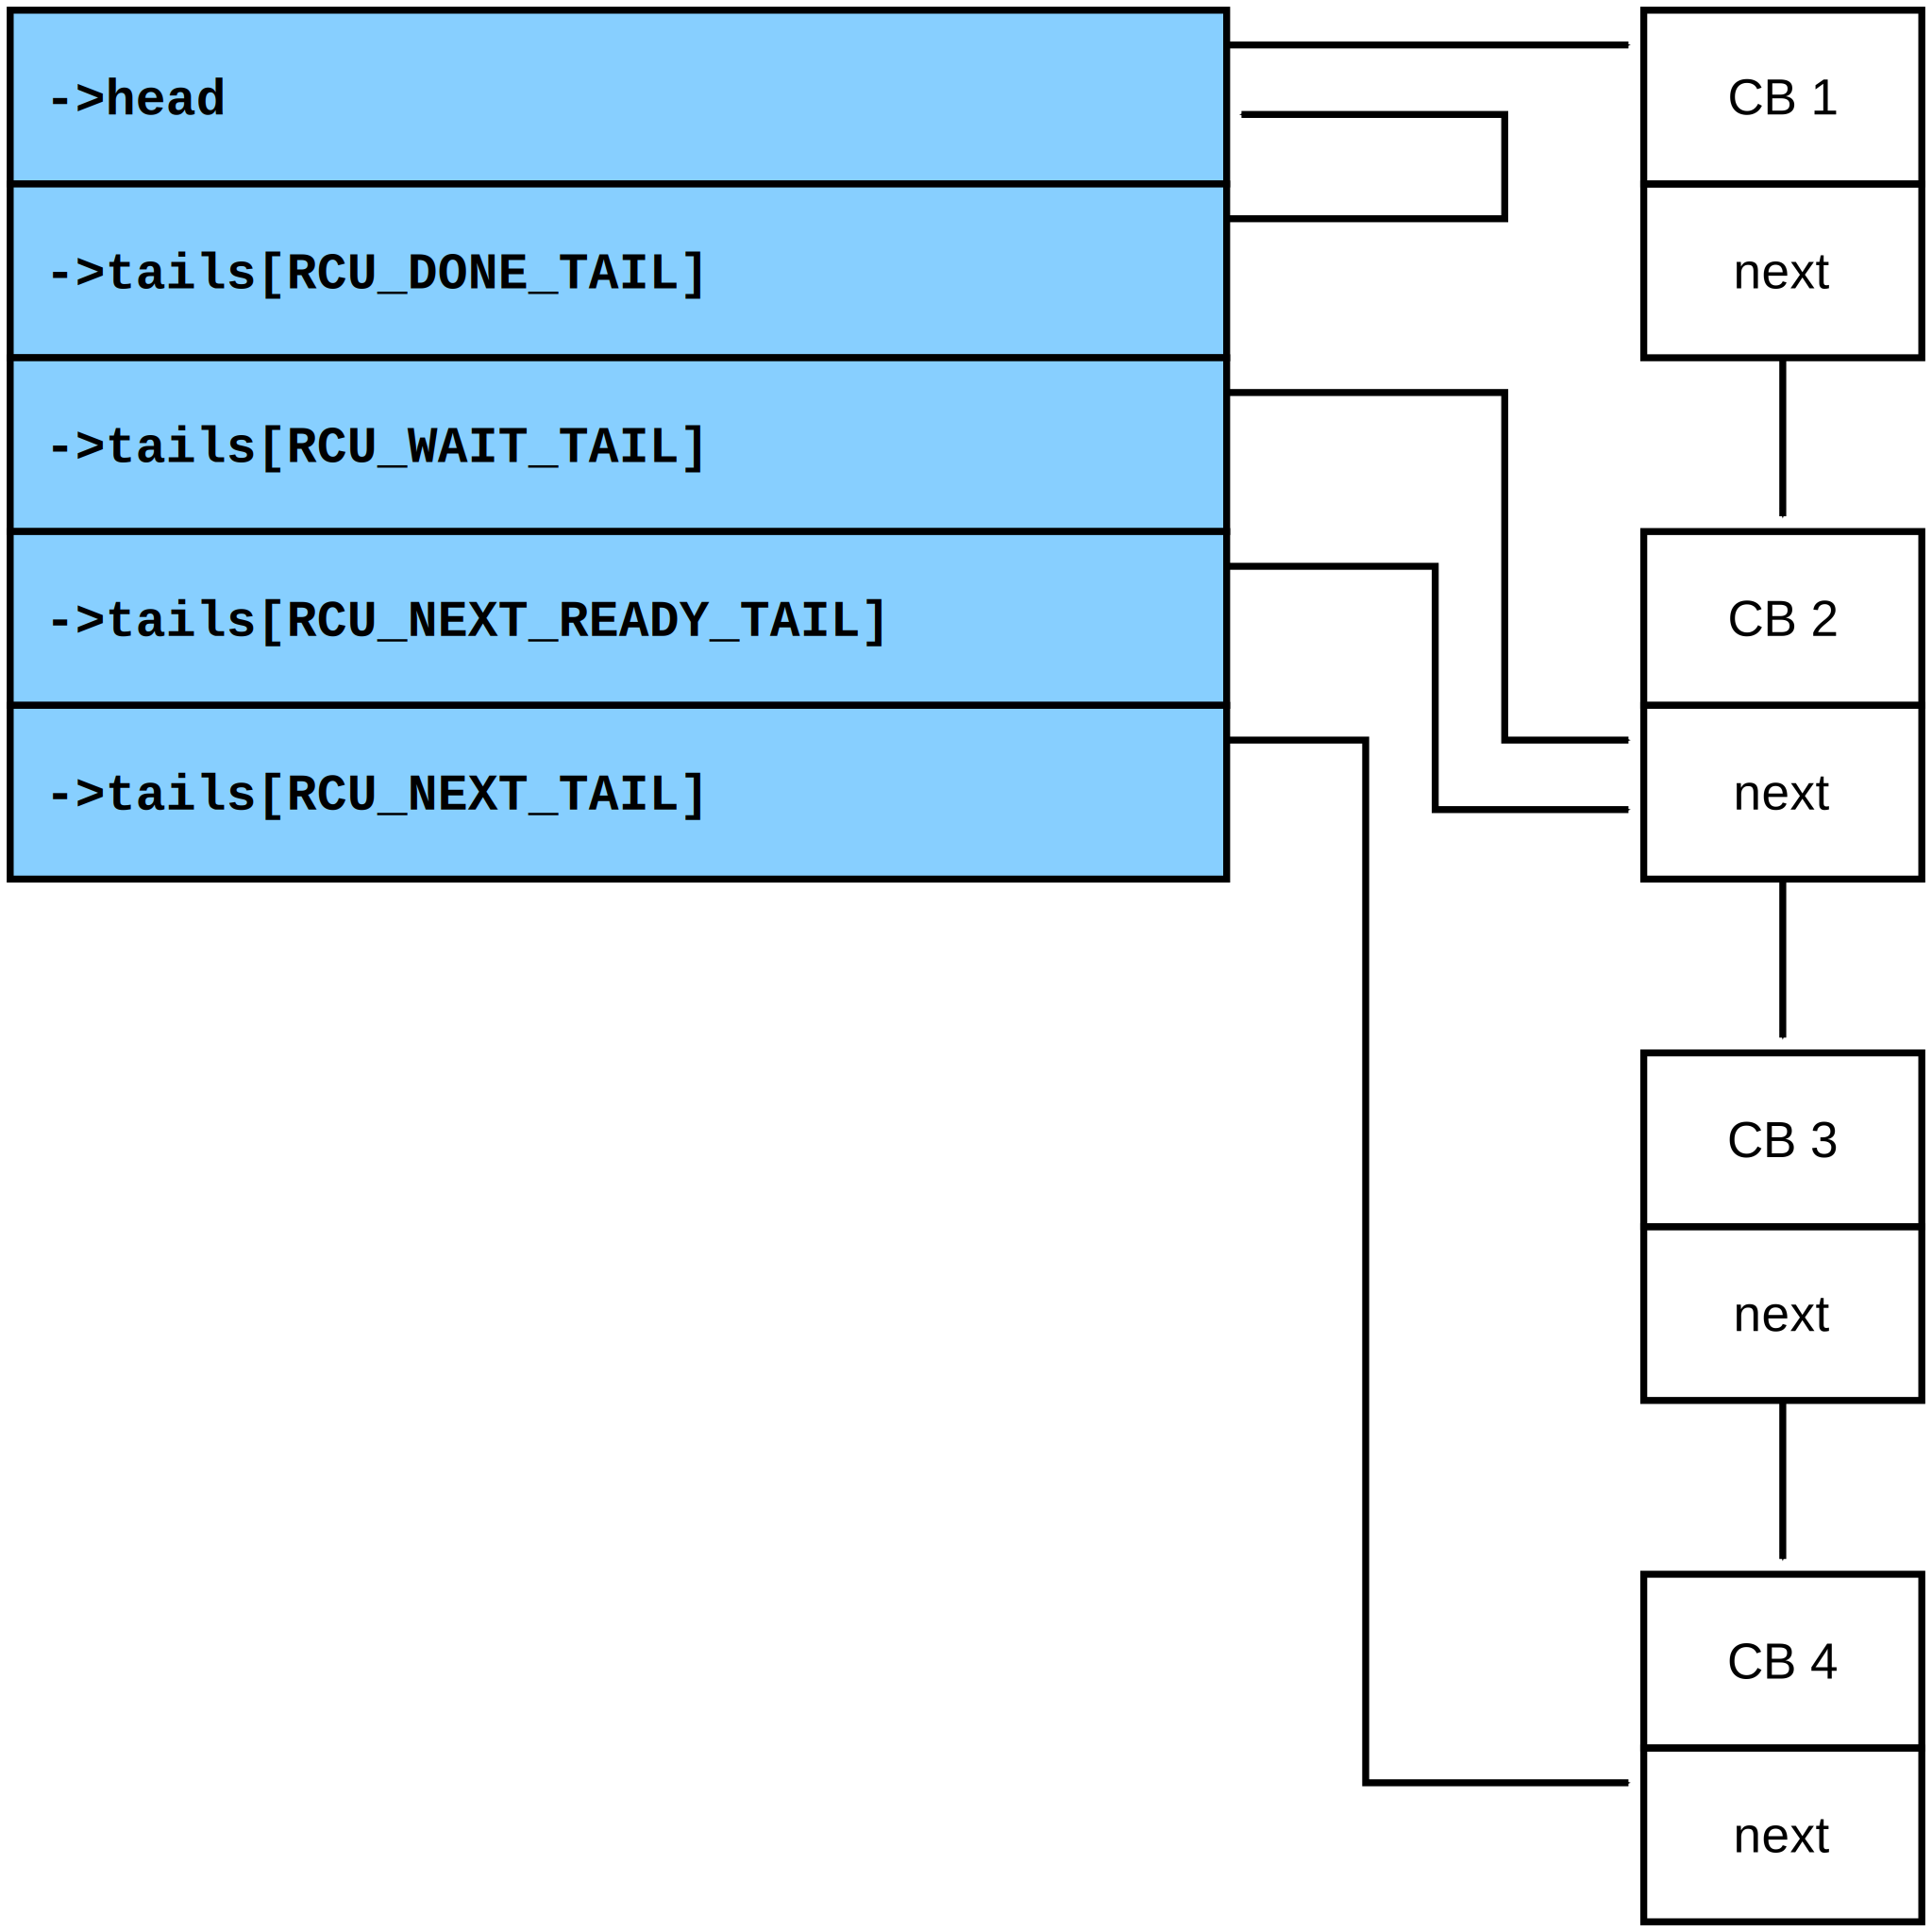
\includegraphics{rcu/design/nxtlist}}
\end{center}

In this figure, the \co{->head} pointer references the first RCU callback
in the list.
The \co{->tails[RCU_DONE_TAIL]} array element references the
\co{->head} pointer itself, indicating that none of the callbacks is
ready to invoke.
The \co{->tails[RCU_WAIT_TAIL]} array element references
callback CB~2's \co{->next} pointer, which indicates that CB~1 and CB~2
are both waiting on the current grace period, give or take possible
disagreements about exactly which grace period is the current one.
The
\co{->tails[RCU_NEXT_READY_TAIL]} array element references the same RCU
callback that \co{->tails[RCU_WAIT_TAIL]} does, which indicates that
there are no callbacks waiting on the next RCU grace period.
The
\co{->tails[RCU_NEXT_TAIL]} array element references CB~4's \co{->next}
pointer, indicating that all the remaining RCU callbacks have not yet
been assigned to an RCU grace period.
Note that the
\co{->tails[RCU_NEXT_TAIL]} array element always references the last RCU
callback's \co{->next} pointer unless the callback list is empty, in
which case it references the \co{->head} pointer.

There is one additional important special case for the
\co{->tails[RCU_NEXT_TAIL]} array element:
It can be \co{NULL} when this
list is \emph{disabled}.
Lists are disabled when the corresponding CPU is
offline or when the corresponding CPU's callbacks are offloaded to a
kthread, both of which are described elsewhere.

CPUs advance their callbacks from the \co{RCU_NEXT_TAIL} to the
\co{RCU_NEXT_READY_TAIL} to the \co{RCU_WAIT_TAIL} to the
\co{RCU_DONE_TAIL} list segments as grace periods advance.

The \co{->gp_seq[]} array records grace-period numbers corresponding to
the list segments.
This is what allows different CPUs to have different
ideas as to which is the current grace period while still avoiding
premature invocation of their callbacks.
In particular, this allows CPUs
that go idle for extended periods to determine which of their callbacks
are ready to be invoked after reawakening.

The \co{->len} counter contains the number of callbacks in \co{->head},
and the \co{->len_lazy} contains the number of those callbacks that are
known to only free memory, and whose invocation can therefore be safely
deferred.

\begin{Note}
   Important:

   It is the \co{->len} field that determines whether or
   not there are callbacks associated with this \co{rcu_segcblist}
   structure, \emph{not} the \co{->head} pointer.
   The reason for this is that all
   the ready-to-invoke callbacks (that is, those in the \co{RCU_DONE_TAIL}
   segment) are extracted all at once at callback-invocation time
   (\co{rcu_do_batch}), due to which \co{->head} may be set to \co{NULL} if there
   are no not-done callbacks remaining in the \co{rcu_segcblist}.
   If
   callback invocation must be postponed, for example, because a
   high-priority process just woke up on this CPU, then the remaining
   callbacks are placed back on the \co{RCU_DONE_TAIL} segment and
   \co{->head} once again points to the start of the segment.
   In short, the
   head field can briefly be \co{NULL} even though the CPU has callbacks
   present the entire time.
   Therefore, it is not appropriate to test the
   \co{->head} pointer for \co{NULL}.
\end{Note}

In contrast, the \co{->len} and \co{->len_lazy} counts are adjusted only
after the corresponding callbacks have been invoked.
This means that the
\co{->len} count is zero only if the \co{rcu_segcblist} structure really
is devoid of callbacks.
Of course, off-CPU sampling of the \co{->len}
count requires careful use of appropriate synchronization, for example,
memory barriers.
This synchronization can be a bit subtle, particularly
in the case of \co{rcu_barrier()}.

\subsubsection{The \texttt{rcu\_data} Structure}

The \co{rcu_data} maintains the per-CPU state for the RCU subsystem.
The
fields in this structure may be accessed only from the corresponding CPU
(and from tracing) unless otherwise stated.
This structure is the focus
of quiescent-state detection and RCU callback queuing.
It also tracks
its relationship to the corresponding leaf \co{rcu_node} structure to
allow more-efficient propagation of quiescent states up the \co{rcu_node}
combining tree.
Like the \co{rcu_node} structure, it provides a local
copy of the grace-period information to allow for-free synchronized
access to this information from the corresponding CPU\@.
Finally, this
structure records past dyntick-idle state for the corresponding CPU and
also tracks statistics.

The \co{rcu_data} structure's fields are discussed, singly and in groups,
in the following sections.

\paragraph{Connection to Other Data Structures}

This portion of the \co{rcu_data} structure is declared as follows:

\begin{VerbatimN}
		int cpu;
		struct rcu_node *mynode;
		unsigned long grpmask;
		bool beenonline;
\end{VerbatimN}

The \co{->cpu} field contains the number of the corresponding CPU and the
\co{->mynode} field references the corresponding \co{rcu_node} structure.
The \co{->mynode} is used to propagate quiescent states up the combining
tree.
These two fields are constant and therefore do not require
synchronization.

The \co{->grpmask} field indicates the bit in the \co{->mynode->qsmask}
corresponding to this \co{rcu_data} structure, and is also used when
propagating quiescent states.
The \co{->beenonline} flag is set whenever
the corresponding CPU comes online, which means that the debugfs tracing
need not dump out any \co{rcu_data} structure for which this flag is not
set.

\paragraph{Quiescent-State and Grace-Period Tracking}

This portion of the \co{rcu_data} structure is declared as follows:

\begin{VerbatimN}
		unsigned long gp_seq;
		unsigned long gp_seq_needed;
		bool cpu_no_qs;
		bool core_needs_qs;
		bool gpwrap;
\end{VerbatimN}

The \co{->gp_seq} field is the counterpart of the field of the same name
in the \co{rcu_state} and \co{rcu_node} structures.
The
\co{->gp_seq_needed} field is the counterpart of the field of the same
name in the \co{rcu_node} structure.
They may each lag up to one behind their
\co{rcu_node} counterparts, but in \co{CONFIG_NO_HZ_IDLE} and
\co{CONFIG_NO_HZ_FULL} kernels can lag arbitrarily far behind for CPUs in
dyntick-idle mode (but these counters will catch up upon exit from
dyntick-idle mode).
If the lower two bits of a given \co{rcu_data}
structure's \co{->gp_seq} are zero, then this \co{rcu_data} structure
believes that RCU is idle.

\QuickQuiz{
  All this replication of the grace period numbers can only cause
  massive confusion.
  Why not just keep a global sequence number and be
  done with it???
}\QuickQuizAnswer{
  Because if there was only a single global sequence numbers, there
  would need to be a single global lock to allow safely accessing and
  updating it.
  And if we are not going to have a single global lock, we
  need to carefully manage the numbers on a per-node basis.
  Recall from
  the answer to a previous Quick Quiz that the consequences of applying
  a previously sampled quiescent state to the wrong grace period are
  quite severe.
}\QuickQuizEnd

The \co{->cpu_no_qs} flag indicates that the CPU has not yet passed
through a quiescent state, while the \co{->core_needs_qs} flag indicates
that the RCU core needs a quiescent state from the corresponding CPU\@.
The \co{->gpwrap} field indicates that the corresponding CPU has remained
idle for so long that the \co{gp_seq} counter is in danger of overflow,
which will cause the CPU to disregard the values of its counters on its
next exit from idle.

\paragraph{RCU Callback Handling}

In the absence of CPU-hotplug events, RCU callbacks are invoked by the
same CPU that registered them.
This is strictly a cache-locality
optimization: callbacks can and do get invoked on CPUs other than the
one that registered them.
After all, if the CPU that registered a given
callback has gone offline before the callback can be invoked, there
really is no other choice.

This portion of the \co{rcu_data} structure is declared as follows:

\begin{VerbatimN}
	struct rcu_segcblist cblist;
	long qlen_last_fqs_check;
	unsigned long n_cbs_invoked;
	unsigned long n_nocbs_invoked;
	unsigned long n_cbs_orphaned;
	unsigned long n_cbs_adopted;
	unsigned long n_force_qs_snap;
	long blimit;
\end{VerbatimN}

The \co{->cblist} structure is the segmented callback list described
earlier.
The CPU advances the callbacks in its \co{rcu_data} structure
whenever it notices that another RCU grace period has completed.
The CPU
detects the completion of an RCU grace period by noticing that the value
of its \co{rcu_data} structure's \co{->gp_seq} field differs from that of
its leaf \co{rcu_node} structure.
Recall that each \co{rcu_node}
structure's \co{->gp_seq} field is updated at the beginnings and ends of
each grace period.

The \co{->qlen_last_fqs_check} and \co{->n_force_qs_snap} coordinate the
forcing of quiescent states from \co{call_rcu()} and friends when
callback lists grow excessively long.

The \co{->n_cbs_invoked}, \co{->n_cbs_orphaned}, and \co{->n_cbs_adopted}
fields count the number of callbacks invoked, sent to other CPUs when
this CPU goes offline, and received from other CPUs when those other
CPUs go offline.
The \co{->n_nocbs_invoked} is used when the CPU's
callbacks are offloaded to a kthread.

Finally, the \co{->blimit} counter is the maximum number of RCU callbacks
that may be invoked at a given time.

\paragraph{Dyntick-Idle Handling}

This portion of the \co{rcu_data} structure is declared as follows:

\begin{VerbatimN}
		int watching_snap;
		unsigned long dynticks_fqs;
\end{VerbatimN}

The \co{->watching_snap} field is used to take a snapshot of the
corresponding CPU's dyntick-idle state when forcing quiescent states,
and is therefore accessed from other CPUs.
Finally, the
\co{->dynticks_fqs} field is used to count the number of times this CPU
is determined to be in dyntick-idle state, and is used for tracing and
debugging purposes.

This portion of the \co{rcu_data} structure is declared as follows:

\begin{VerbatimN}
		long nesting;
		long nmi_nesting;
		atomic_t dynticks;
		bool rcu_need_heavy_qs;
		bool rcu_urgent_qs;
\end{VerbatimN}

These fields in the \co{rcu_data} structure maintain the per-CPU dyntick-idle
state for the corresponding CPU\@.
The fields may be accessed only from
the corresponding CPU (and from tracing) unless otherwise stated.

The \co{->nesting} field counts the nesting depth of process
execution, so that in normal circumstances this counter has value zero
or one.
NMIs, irqs, and tracers are counted by the
\co{->nmi_nesting} field.
Because NMIs cannot be masked, changes
to this variable have to be undertaken carefully using an algorithm
provided by Andy Lutomirski.
The initial transition from idle adds one,
and nested transitions add two, so that a nesting level of five is
represented by a \co{->nmi_nesting} value of nine.
This counter
can therefore be thought of as counting the number of reasons why this
CPU cannot be permitted to enter dyntick-idle mode, aside from
process-level transitions.

However, it turns out that when running in non-idle kernel context, the
Linux kernel is fully capable of entering interrupt handlers that never
exit and perhaps also vice versa.
Therefore, whenever the
\co{->nesting} field is incremented up from zero, the
\co{->nmi_nesting} field is set to a large positive number, and
whenever the \co{->nesting} field is decremented down to zero,
the \co{->nmi_nesting} field is set to zero.
Assuming that
the number of misnested interrupts is not sufficient to overflow the
counter, this approach corrects the \co{->nmi_nesting} field
every time the corresponding CPU enters the idle loop from process
context.

The \co{->dynticks} field counts the corresponding CPU's transitions to
and from either dyntick-idle or user mode, so that this counter has an
even value when the CPU is in dyntick-idle mode or user mode and an odd
value otherwise.
The transitions to/from user mode need to be counted
for user mode adaptive-ticks support (see \path{Documentation/timers/no_hz.rst}).

The \co{->rcu_need_heavy_qs} field is used to record the fact that the
RCU core code would really like to see a quiescent state from the
corresponding CPU, so much so that it is willing to call for
heavy-weight dyntick-counter operations.
This flag is checked by RCU's
context-switch and \co{cond_resched()} code, which provide a momentary
idle sojourn in response.

Finally, the \co{->rcu_urgent_qs} field is used to record the fact that
the RCU core code would really like to see a quiescent state from the
corresponding CPU, with the various other fields indicating just how
badly RCU wants this quiescent state.
This flag is checked by RCU's
context-switch path (\co{rcu_note_context_switch}) and the \co{cond_resched}
code.

\QuickQuiz{
  Why not simply combine the \co{->nesting} and
  \co{->nmi_nesting} counters into a single counter that just
  counts the number of reasons that the corresponding CPU is non-idle?
}\QuickQuizAnswer{
  Because this would fail in the presence of interrupts whose handlers
  never return and of handlers that manage to return from a made-up
  interrupt.
}\QuickQuizEnd

Additional fields are present for some special-purpose builds, and are
discussed separately.

\subsubsection{The \texttt{rcu\_head} Structure}

Each \co{rcu_head} structure represents an RCU callback.
These structures
are normally embedded within RCU-protected data structures whose
algorithms use asynchronous grace periods.
In contrast, when using
algorithms that block waiting for RCU grace periods, RCU users need not
provide \co{rcu_head} structures.

The \co{rcu_head} structure has fields as follows:

\begin{VerbatimN}
		struct rcu_head *next;
		void (*func)(struct rcu_head *head);
\end{VerbatimN}

The \co{->next} field is used to link the \co{rcu_head} structures
together in the lists within the \co{rcu_data} structures.
The \co{->func}
field is a pointer to the function to be called when the callback is
ready to be invoked, and this function is passed a pointer to the
\co{rcu_head} structure.
However, \co{kfree_rcu()} uses the \co{->func}
field to record the offset of the \co{rcu_head} structure within the
enclosing RCU-protected data structure.

Both of these fields are used internally by RCU\@.
From the viewpoint of
RCU users, this structure is an opaque ``cookie''.

\QuickQuiz{
  Given that the callback function \co{->func} is passed a pointer to
  the \co{rcu_head} structure, how is that function supposed to find the
  beginning of the enclosing RCU-protected data structure?
}\QuickQuizAnswer{
  In actual practice, there is a separate callback function per type of
  RCU-protected data structure.
  The callback function can therefore use
  the \co{container_of()} macro in the Linux kernel (or other
  pointer-manipulation facilities in other software environments) to
  find the beginning of the enclosing structure.
}\QuickQuizEnd

\subsubsection{RCU-Specific Fields in the \texttt{task\_struct} Structure}

The \co{CONFIG_PREEMPT_RCU} implementation uses some additional fields in
the \co{task_struct} structure:

\begin{VerbatimN}
	#ifdef CONFIG_PREEMPT_RCU
		int rcu_read_lock_nesting;
		union rcu_special rcu_read_unlock_special;
		struct list_head rcu_node_entry;
		struct rcu_node *rcu_blocked_node;
	#endif /* #ifdef CONFIG_PREEMPT_RCU */
	#ifdef CONFIG_TASKS_RCU
		unsigned long rcu_tasks_nvcsw;
		bool rcu_tasks_holdout;
		struct list_head rcu_tasks_holdout_list;
		int rcu_tasks_idle_cpu;
	#endif /* #ifdef CONFIG_TASKS_RCU */
\end{VerbatimN}

The \co{->rcu_read_lock_nesting} field records the nesting level for RCU
read-side critical sections, and the \co{->rcu_read_unlock_special} field
is a bitmask that records special conditions that require
\co{rcu_read_unlock()} to do additional work.
The \co{->rcu_node_entry}
field is used to form lists of tasks that have blocked within
preemptible-RCU read-side critical sections and the
\co{->rcu_blocked_node} field references the \co{rcu_node} structure whose
list this task is a member of, or \co{NULL} if it is not blocked within a
preemptible-RCU read-side critical section.

The \co{->rcu_tasks_nvcsw} field tracks the number of voluntary context
switches that this task had undergone at the beginning of the current
tasks-RCU grace period, \co{->rcu_tasks_holdout} is set if the current
tasks-RCU grace period is waiting on this task,
\co{->rcu_tasks_holdout_list} is a list element enqueuing this task on
the holdout list, and \co{->rcu_tasks_idle_cpu} tracks which CPU this
idle task is running, but only if the task is currently running, that
is, if the CPU is currently idle.

\subsubsection{Accessor Functions}

The following listing shows the \co{rcu_get_root()},
\co{rcu_for_each_node_breadth_first} and \co{rcu_for_each_leaf_node()}
function and macros:

\begin{VerbatimN}
	static struct rcu_node *rcu_get_root(struct rcu_state *rsp)
	{
		return &rsp->node[0];
	}

	#define rcu_for_each_node_breadth_first(rsp, rnp) \
	        for ((rnp) = &(rsp)->node[0]; \
	             (rnp) < &(rsp)->node[NUM_RCU_NODES]; (rnp)++)

	#define rcu_for_each_leaf_node(rsp, rnp) \
	        for ((rnp) = (rsp)->level[NUM_RCU_LVLS - 1]; \
	             (rnp) < &(rsp)->node[NUM_RCU_NODES]; (rnp)++)
\end{VerbatimN}

The \co{rcu_get_root()} simply returns a pointer to the first element of
the specified \co{rcu_state} structure's \co{->node[]} array, which is the
root \co{rcu_node} structure.

As noted earlier, the \co{rcu_for_each_node_breadth_first()} macro takes
advantage of the layout of the \co{rcu_node} structures in the
\co{rcu_state} structure's \co{->node[]} array, performing a breadth-first
traversal by simply traversing the array in order.
Similarly, the
\co{rcu_for_each_leaf_node()} macro traverses only the last part of the
array, thus traversing only the leaf \co{rcu_node} structures.

\QuickQuiz{
  What does \co{rcu_for_each_leaf_node()} do if the \co{rcu_node} tree
  contains only a single node?
}\QuickQuizAnswer{
  In the single-node case, \co{rcu_for_each_leaf_node()} traverses the
  single node.
}\QuickQuizEnd

\subsection{Summary}

So the state of RCU is represented by an \co{rcu_state} structure, which
contains a combining tree of \co{rcu_node} and \co{rcu_data} structures.
Finally, in \co{CONFIG_NO_HZ_IDLE} kernels, each CPU's dyntick-idle state
is tracked by dynticks-related fields in the \co{rcu_data} structure.
If
you made it this far, you are well prepared to read the code
walkthroughs in the other articles in this series.

\subsection{Acknowledgments}

I owe thanks to Cyrill Gorcunov, Mathieu Desnoyers, Dhaval Giani, Paul
Turner, Abhishek Srivastava, Matt Kowalczyk, and Serge Hallyn for
helping me get this document into a more human-readable state.

\subsection{Legal Statement}

This work represents the view of the author and does not necessarily
represent the view of IBM\@.

Linux is a registered trademark of Linus Torvalds.

Other company, product, and service names may be trademarks or service
marks of others.
